% !TEX root = ../my-thesis.tex
%
\chapter{Model Based Clustering}
\label{sec:clustering}

\cleanchapterquote{\ldots savoir discerner les plus importantes de
celles qui sont seulement accessoires, les balancer toutes convenablement entre elles, afin de parvenir, par les moyens les plus faciles, au
meilleur r\'esultat, tel doit \^etre le principal talent de l'homme\ldots}{Nicolas L\'eonard Sadi Carnot}{(French physicist, 1796-1832)}


\section{Introduction}
\label{sec:clustering:intro}

In this chapter, we present a model-based clustering scheme to build a piecewise reconstruction of a function $f$ from a set of observations $\data$. Recalling what has been discussed in \S\ref{sec:sota_2}, the goal is to construct a piecewise surrogate model of the form:

\begin{equation}
  \tilde{f}(\bx; \boldsymbol{\beta}, \mathcal{P}) = \sum_{l=1}^L \mathbb{I}_{\Omega_l}(\bx; \boldsymbol{\gamma}) \tilde{f}_l(\bx; \boldsymbol{\beta}_l) \;,
\end{equation}

where $\mathbb{I}_{\Omega_l}(\bx; \boldsymbol{\gamma})$ is the indicator function of the cluster $l$, which depends on the classifier hyperparameters $\boldsymbol{\gamma}$, and $\tilde{f}_l(\bx; \boldsymbol{\beta}_l)$ is the local surrogate model corresponding to cluster $l$, which depends on the local regressor hyperparameters $\boldsymbol{\beta}_l$. In \S\ref{sec:sota_2}, we have shown that solving this problem \blue{implies} solving a clustering problem, in which we need to identify a good \blue{partition $\mathcal{P}$} of the observations $\data$ into $L$ clusters, and a classifier $c(\cdot; \boldsymbol{\gamma})$ that can separate these clusters, and local regressors $\tilde{f}_l(\cdot; \boldsymbol{\beta}_l)$ that can fit the observations in each cluster. 

\smallskip
This problem is particularly challenging as one needs to select values for the following hyperparameters: $\boldsymbol{\beta}, \boldsymbol{\gamma}, \mathbf{z}$. In this chapter, we shall adopt an optimization approach to solve this problem, in which we search for the optimal values of these hyperparameters by maximizing a global score function. The first part of the next section is dedicated to the definition of an appropriate score function that can capture the performance of the global piecewise reconstruction. 

\smallskip
On the other hand, even if such a score function, here termed $S_{\mathrm{global}}(\boldsymbol{\beta}, \boldsymbol{\gamma}, \mathbf{z})$, is well defined, it is not trivial to optimize it with respect to the hyperparameters $\boldsymbol{\beta}, \boldsymbol{\gamma}, \mathbf{z}$, as the optimization problem is non-convex and very high-dimensional. For this reason, we search for an alternate iterative optimization scheme, in which we iteratively update the cluster labels $\mathbf{z}$, the classifier hyperparameters $\boldsymbol{\gamma}$ and the surrogate model hyperparameters $\boldsymbol{\beta}$ until convergence. 

\smallskip
We can start with a simple clustering $\mathbf{z}^{(0)}$, such as~\cite{Sudret2023,lloyd1982least}, and then iteratively refine it based on the performance of the surrogate model to obtain more accurate predictions. 


\begin{figure}[htbp]
    \centering
    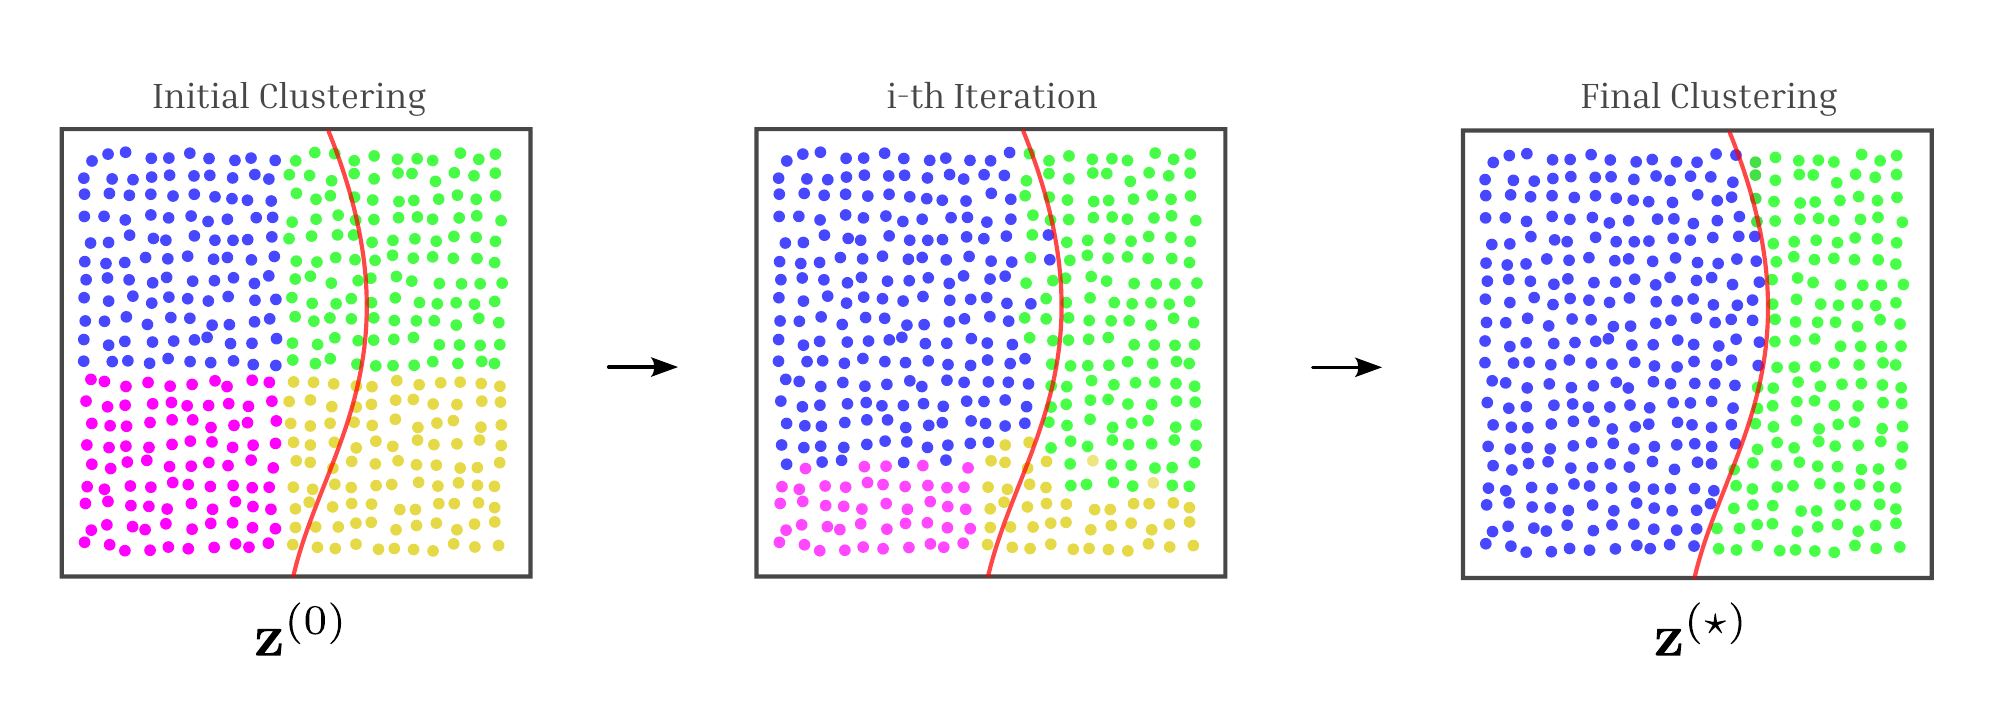
\includegraphics[width=\textwidth]{figures/clustering/Evolution.png}
    \caption{Schematic representation of the proposed model-based clustering algorithm. The red line represents a possible discontinuity and points represent the training data, clustered according to their color.}
    \label{fig:sota_2:model_based_clustering}
\end{figure}

Fig.~\ref{fig:sota_2:model_based_clustering} provides a schematic representation of the proposed \blue{clustering} algorithm \blue{for a function with a discontinuity represented by the red line}. \blue{The clustering is initialized} with a simple and possibly bad clustering $\mathbf{z}^{(0)}$, and then \blue{it is} iteratively refined based \blue{on the score function $S_{\mathrm{global}}(\boldsymbol{\beta}, \boldsymbol{\gamma}, \mathbf{z})$, reaching the final solution $\mathbf{z}^{(\star)}$.} The question is how to perform this \blue{iterative update}, i.e., how to update the cluster labels $\mathbf{z}$, the classifier hyperparameters $\boldsymbol{\gamma}$ and the surrogate model hyperparameters $\boldsymbol{\beta}$ at each iteration.


\section{Model Based Clustering Scheme}
\label{sc:mc_algorithm}

\blue{In this section, we present the model-based clustering scheme. In \S\ref{sec:clustering:mb:score} we define the global score function $S_{\mathrm{global}}(\boldsymbol{\beta}, \boldsymbol{\gamma}, \mathbf{z})$, in \S\ref{sec:clustering:mb:it} we present the iterative updating scheme, and in \S\ref{sec:clustering:mb:reduction_merging} we detail how to reduce the number of clusters by purging small clusters and merging clusters that belong to the same smooth subregion. Finally, in \S\ref{sc:convergence} we prove that, under some reasonable assumptions, the algorithm converges in a finite number of steps.}


\subsection{Score Function Definition}
\label{sec:clustering:mb:score}

Defining an appropriate score function is not trivial, since we want to capture the global performance of a series of local regressors. To start, we have shown in Eq.~\eqref{eq:sota_2:error_decomposition} that the global error of a piecewise surrogate model can be decomposed into the sum of the local errors of the local regressors on their corresponding clusters. \blue{A first approach is to use} a proxy score function based on replacing the integral \blue{in Eq.~\eqref{eq:sota_2:error_decomposition}} with a sum over the observations \blue{of each cluster}, and the true function $f$ with the observed values $y_i$. Although appealing, this score function is a poor choice; training local regressors to minimize an error over the observations is known to be prone to overfitting. Luckily, practitioners are very well aware of this issue and have developed tailored score functions to be maximized during model selections. We have already introduced these functions in Eq.~\eqref{eq:sota_2:score_functions}, and termed them $S(\boldsymbol{\beta},\data)$. Since these are well established in the literature and constantly used in practice, we propose to use them as our score function by summing the local scores, i.e.,

\begin{equation}
  S_{\mathrm{global}}(\boldsymbol{\beta}, \mathbf{z}) = \summ{l}{1}{L} S(\boldsymbol{\beta}_l, \data_l(\mathbf{z})) \;.
  \label{eq:clustering:global_score}
\end{equation}

In the above equation, $\data_l(\mathbf{z})$ is the subset of observations belonging to cluster $l$ according to the cluster assignments $\mathbf{z}$, and $\boldsymbol{\beta}_l$ are the hyperparameters of the local regressor corresponding to cluster $l$, while $\boldsymbol{\beta} = \{\boldsymbol{\beta}_1, \ldots, \boldsymbol{\beta}_L\}$ is the set of all local regressor hyperparameters. Notice that the advantage of using the score function in Eq.~\eqref{eq:clustering:global_score} is that each local regressor can be trained independently by maximizing its local score. To us, this is a crucial property, as we are not altering well-established training procedures and can leverage existing codes, even gradient-based optimization algorithms, to perform model selection and define $\boldsymbol{\beta}_l$. To see this, we consider the gradient of the global score with respect to the hyperparameters of a local regressor $l$, $\boldsymbol{\beta}_l$,

\begin{equation}
  \left.
  \begin{aligned}
    \nabla_{\boldsymbol{\beta}_l} S_{\mathrm{global}}(\boldsymbol{\beta}, \mathbf{z}) =& \nabla_{\boldsymbol{\beta}_l} S(\boldsymbol{\beta}_l, \data_l(\mathbf{z})) + \sum_{l^\prime \neq l} \nabla_{\boldsymbol{\beta}_l} S(\boldsymbol{\beta}_{l^\prime}, \data_{l^\prime}(\mathbf{z}))\\
    =& \nabla_{\boldsymbol{\beta}_l} S(\boldsymbol{\beta}_l, \data_l(\mathbf{z}))\;.
  \end{aligned}
  \right.
\end{equation}

As we can see, the gradient of the global score with respect to the hyperparameters of a local regressor $l$ is equal to the gradient of the local score of that regressor, and does not depend on the other local regressors. This means that we can train each local regressor independently by maximizing its local score, which is a crucial property for the computational efficiency of our approach as it allows for parallel training. 

\subsection{Iterative Scheme}
\label{sec:clustering:mb:it}

\blue{We now introduce here the iterative updating strategy. It is based on the improvement of $S_{\mathrm{global}}(\boldsymbol{\beta}, \mathbf{z})$ when the $i$-th observation changes from its current cluster $l$ to a new cluster $l^{\prime}$. The associated change in global score function is denoted as $\Delta S (l \rightarrow l^\prime; \bx_i, \mathbf{z}, \boldsymbol{\beta})$ and writes:}

\begin{equation}
  \left.
  \begin{aligned}
    \Delta S (l \rightarrow l^\prime; \bx_i, \mathbf{z}, \boldsymbol{\beta}) =&\ S(\boldsymbol{\beta}_{l^\prime}, \data_{l^\prime}(\mathbf{z}) \cup \mathbf{d}_i) + S(\boldsymbol{\beta}_{l}, \data_{l}(\mathbf{z}) \setminus \mathbf{d}_i)
    \\ &- S(\boldsymbol{\beta}_{l^\prime}, \data_{l^\prime}(\mathbf{z})) - S(\boldsymbol{\beta}_{l}, \data_{l}(\mathbf{z})) \;.
  \end{aligned}
  \right.
  \label{eq:clustering:change_score}
\end{equation}

Unless required, in the following sections we will drop the explicit dependence of $\Delta S (\cdot)$ on $\mathbf{z}$ and $\boldsymbol{\beta}$ to simplify the notation.
\blue{Eq.~\eqref{eq:clustering:change_score} assumes that the hyperparameters $\boldsymbol{\beta}$ remain fixed for each local regressor during the evaluation of the change of score. This assumption, although essential for fast and efficient query of $\Delta S (l \rightarrow l^\prime; \bx_i)$, does not affect the convergence of the iterative clustering algorithm, as shown in \S\ref{sc:convergence}. The iterative membership update criterion consists of updating $\mathbf{z}^{(t)} \rightarrow \mathbf{z}^{(t+1)}$ by promoting membership updates that lead to an increase in the global score, i.e., $S(\boldsymbol{\beta}^{(t)}, \mathbf{z}^{(t+1)}) > S(\boldsymbol{\beta}^{(t)}, \mathbf{z}^{(t)})$, and then updating the local regressor hyperparameters $\boldsymbol{\beta}^{(t)} \rightarrow \boldsymbol{\beta}^{(t+1)}$ by maximizing the local scores on the new clusters.}

\smallskip
Notice we only calculate the change in global score when a single point per cluster changes its membership. Indeed, given a general update $\mathbf{z}^{(t)} \rightarrow \mathbf{z}^{(t+1)}$, the resulting change in global score is not equal to the sum of the individual $\Delta S (\cdot)$,

\begin{equation}
  S(\boldsymbol{\beta}^{(t)}, \mathbf{z}^{(t+1)}) - S(\boldsymbol{\beta}^{(t)}, \mathbf{z}^{(t)}) \neq \displaystyle\sum_{i \in \mathcal{O}} \Delta S (z_i^{(t)} \rightarrow z_i^{(t+1)}; \bx_i) \;.
\end{equation}

To keep the problem tractable while still allowing batch membership updates we deliberately introduce the independent $\Delta S (\cdot)$ approximation but restrict the set of points that can change their membership to a subset of the total, $\mathcal{O}_{\mathrm{update}} \subset \mathcal{O}$.

\smallskip
Finally, details on the specific expression of $\Delta S (l \rightarrow l^\prime; \bx_i)$ for \glspl{gp} and \glspl{pce} are deferred to \S\ref{sc:score_functions}.

\smallskip
\blue{On the one hand, the above-mentioned update strategy constitutes the core of our model-based clustering scheme. On the other hand, it is prone to severe overfitting issues, which will be illustrated on a simple example.}

\begin{figure}[htbp]
  \centering
  \begin{subfigure}{0.49\textwidth}
    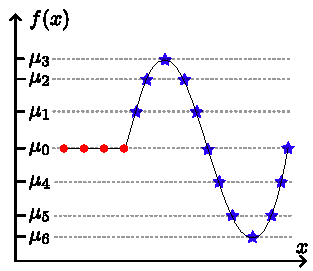
\includegraphics[width=\textwidth]{figures/clustering/goodClustering.pdf}
    \caption{Correct clustering.}
    \label{fig:clustering:bad_clustering_1}
  \end{subfigure}
  \hfill
  \begin{subfigure}{0.49\textwidth}
    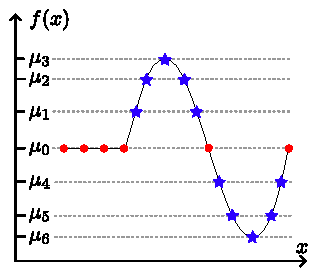
\includegraphics[width=\textwidth]{figures/clustering/badClustering.pdf}
    \caption{Incorrect clustering.}
    \label{fig:clustering:bad_clustering_2}
  \end{subfigure}
  \caption{Visual representation of a good and a bad clustering. The bad clustering, although leading to a higher global score, creates disconnected clusters that lead to a poor reconstruction of the subdomains. Points are colored according to their cluster membership.}
  \label{fig:clustering:bad_clustering}
\end{figure}

In Fig.~\ref{fig:clustering:bad_clustering} we show a visual representation of what overfitting can look like in our setting. In the left panel, we have a good clustering of the observations, where each cluster corresponds to a connected region of the input space. However, the clustering in Fig.~\ref{fig:clustering:bad_clustering_1} does not maximize the global score; it is the clustering in Fig.~\ref{fig:clustering:bad_clustering_2} that does it. The global score is higher in the second case because one local regressor is a simple constant (fixed mean and very low variance) that fits perfectly observations close to its prior mean. However, this clustering is not desirable as it is disconnected and does not lead to a good reconstruction of the subdomains. This is a clear example of overfitting, and we must prevent it by discouraging membership updates that lead to disconnected clusters. 

\smallskip
What Eq.~\eqref{eq:clustering:global_score} is missing is a term that captures the performance of the classifier in separating the clusters. Rather than adding this term to the global score, in Eq.~\eqref{eq:clustering:global_score}, we propose to use it to modify the membership update criterion defined in Eq.~\eqref{eq:clustering:change_score}. In particular, Eq.~\eqref{eq:clustering:change_score} captures the gain in global score when updating memberships and $\mathbb{P}_{\mathrm{CLS}}(\cdot)$ computes whether the new membership is admissible according to the classifier (higher probability for points close to the boundaries and lower probability for points far from the boundaries). We can combine these two to formulate a stochastic membership update criterion, in which the probability of changing the membership of an observation $i$ to a cluster $l$ is defined as follows,

\begin{equation}
  \left.
\begin{aligned}
  &\mathbb{P}(l \rightarrow l^{\prime} \mid \bx_i, \mathbf{z}, T) \propto \exp \left( \dfrac{1}{T}\Delta S (l \rightarrow l^\prime; \bx_i)\right) \, h\left(\mathbb{P}_{\mathrm{CLS}}(l^\prime \mid \bx_i, \boldsymbol{\gamma}) \right) \;,\\
  &\text{With: } \sum_{l^\prime=1}^L \mathbb{P}(l \rightarrow l^\prime \mid \bx_i, \mathbf{z}, T) = 1 \;.
\end{aligned}
  \right.
  \label{eq:clustering:membership_update_prob}
\end{equation}

In the above equation, $T$ is a temperature parameter and $h(\cdot)$ is an activation function that sets to $0$ updates with a probability less than a user-defined threshold $h_{\min}$ (we usually set $h_{\min} = 0.05$ in our tests). The term inside the exponential captures how much a membership update is desirable in terms of global score, while the term $h\left(\mathbb{P}_{\mathrm{CLS}}(l \mid \bx_i, \boldsymbol{\gamma}) \right)$ captures whether the new membership is admissible according to the classifier while $h(\cdot)$ prevents the first term from dominating when $T\rightarrow 0$ for a membership update that is not admissible. Moving towards a stochastic optimization scheme introduces a new degree of freedom that balances exploration and exploitation. When $T$ is high, the classifier term dominates and boundary points randomly change their membership, allowing for a more efficient exploration of the clustering space. When $T$ is low, the global score term dominates and only updates that lead to an increase in global score are performed, leading to a more efficient exploitation of the clustering space.


\smallskip
In practice, we always consider two scenarios. In the first scenario, we set $T=0$, leading to a deterministic optimization scheme in which only updates that lead to an increase in global score are performed. In the second scenario, we set $T>0$, decreasing it by a factor $\alpha_T < 1$ (we choose 0.99) at each iteration, leading to a stochastic optimization scheme. We shall discuss the choice of $T$ in more detail when we discuss the initial partitioning of the input space.

\smallskip
Notice that since Eq.~\eqref{eq:clustering:membership_update_prob} does not yield the probability of changing the membership of an observation $i$ to any cluster, but only the probability of changing the membership of an observation $i$ to a specific cluster $l^\prime$, which can be also equal to its current cluster $l$, we can derive the probability of changing the membership of an observation $i$ from its current cluster $l$ to any other cluster as follows,

\begin{equation}
  \mathbb{P}(l^\prime \neq l \mid \bx_i, \mathbf{z}, T) = 1 - \mathbb{P}(l \rightarrow l \mid \bx_i, \mathbf{z}, T) \;.
  \label{eq:clustering:prob_change_membership}
\end{equation}

With Eq.~\eqref{eq:clustering:prob_change_membership} we can now formulate a stochastic optimization scheme, reported in Algorithm~\ref{alg:clustering:model_clustering}. For the sake of notational clarity, we introduce $\mathcal{O} = \{1, \ldots, \nobs\}$ as the set of indices of the observations in $\data$, not to be confused with the observation operator introduced in \S\ref{sec:sota_2}.

\begin{algorithm}[htbp]
  \caption{Model-Based Clustering}
  \label{alg:clustering:model_clustering}
  \begin{algorithmic}[1]
    \Require Initial clustering $\mathbf{z}$, local regressor parameters $\boldsymbol{\beta}$, classifier parameters $\boldsymbol{\gamma}$, temperature $T$.
    \Ensure Final $\mathbf{z}$, $\boldsymbol{\beta}$, $\boldsymbol{\gamma}$.
    \While{not converged}
      \State Compute transition probabilities for all points $i \in \mathcal{O}$ via Eq.~\eqref{eq:clustering:prob_change_membership}.
      \State Sample a subset $\mathcal{O}_{\mathrm{update}}$ of size $N_{\mathrm{update}} \leq N$ based on these probabilities.
      \For{$i \in \mathcal{O}_{\mathrm{update}}$}
        \State Sample and update membership: $l^\prime \sim \mathbb{P}( \cdot \mid \bx_i, \mathbf{z}, T)$.
      \EndFor
      \State Update local regressors $\forall l$: $\boldsymbol{\beta}_l \gets \argmax_{\boldsymbol{\beta}_l} S(\boldsymbol{\beta}_l, \mathcal{D}_l(\mathbf{z}))$.
      \State Retrain the classifier.
      \State Decrease the temperature $T \gets \alpha_T T$.
    \EndWhile
  \end{algorithmic}
\end{algorithm}

Alg.~\ref{alg:clustering:model_clustering} describes the model based clustering scheme. It runs an iterative optimization process until a convergence criterion is met. At each iteration, it first computes the probability of changing the membership of each observation to any other cluster using Eq.~\eqref{eq:clustering:prob_change_membership}, then it samples a subset of points $\mathcal{O}_{\mathrm{update}}$ according to these probabilities.

\smallskip
After sampling the points that will be allowed to update their membership, we sample a new membership for each of these points from the probabilities defined in Eq.~\eqref{eq:clustering:membership_update_prob}, and if the new membership is different from the current one, we perform the membership update. Finally, at the end of each iteration, we retrain the local models and the classifier on the new clusters by maximizing their local scores and their classification score, respectively.

\smallskip
The cycle continues until a convergence criterion is met, which can be defined based on the change in global score, e.g., $|S_{\mathrm{global}}^{(t+1)} - S_{\mathrm{global}}^{(t)}| \leq \epsilon_S |S_{\mathrm{global}}^{(t)}|$, for some user-defined threshold $\epsilon_S$ or a minimum temperature $T_{\min}$ (equivalent to a maximum number of iterations). In practice, the algorithm usually terminates (no more updates are proposed) in a finite number of steps in most cases, as will be shown in \S\ref{sc:convergence}.

\subsection{Reduction and Merging of Clusters}
\label{sec:clustering:mb:reduction_merging}

\blue{In this section, we detail how to purge clusters with too few points and how to identify and merge two clusters that belong to the same smooth subdomain.}


\subsubsection{Reduction}
A reduction step is a step in which we remove clusters that have a very low number of points, i.e., $|\mathcal{O}_l| < N_{\min}$, for some user-defined threshold $N_{\min}$ (we usually set $N_{\min} = 10$ in our tests). These clusters are not desirable as they are very small and would not lead to a good reconstruction of the subdomains. 

\smallskip
The leftover points are then assigned to the cluster with the highest classifier probability, i.e., $z_i = \argmax_{l} \mathbb{P}_{\mathrm{CLS}}(l \mid \bx_i, \boldsymbol{\gamma})$, and the local regressors and the classifier are retrained on the new clusters. 

\subsubsection{Merging}
In our tests we have also observed that, especially at high temperatures, some clusters tend to mix. This occurs when two clusters $l$ and $l^{\prime}$ are similar, they belong to the same smooth region or are separated by a fake discontinuity. See Fig.~\ref{fig:clustering:confusion} for a visual example.

\begin{figure}
  \centering
  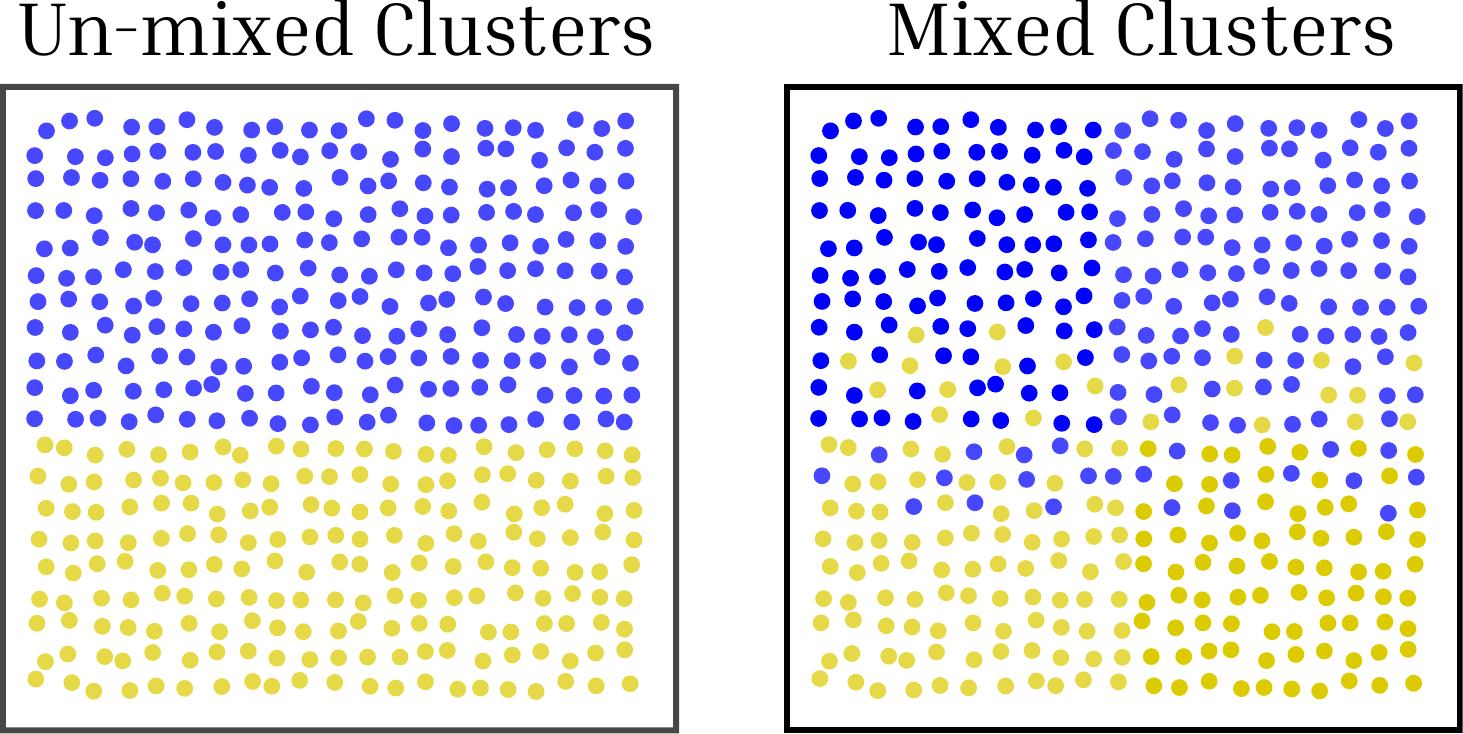
\includegraphics[width=0.5\linewidth]{figures/clustering/confusion.png}
  \caption{A visual representation of two clusters with a clear separation (left) and mixing boundary (right)}
  \label{fig:clustering:confusion}
\end{figure}

Mixing occurs because two local models, for cluster $\mathcal{O}_l$ and $\mathcal{O}_{l^\prime}$, are similar. When this happens the change in score when updating the membership of a point $\bx_i$ from $l$ to $l^\prime$ is equivalent to not updating the membership at all, $\Delta S (l \rightarrow l^{\prime}; \bx_i) \approx 0$ for some $i \in \mathcal{O}_l$. This encourages clusters $\mathcal{O}_l$ and $\mathcal{O}_{l^\prime}$ to progressively exchange random points, starting from their boundaries. This relaxes the classifier margin, promoting more random exchanges. The mechanism continues until the temperature is low enough for small changes in $\Delta S (\cdot)$ to be amplified, leading to un-mixing. 

\smallskip
We can detect these situations by checking a metric called confusion, and defined for a pair of clusters $\mathcal{O}_l$ and $\mathcal{O}_{l^\prime}$ as,

\begin{equation}
  C(l,l^{\prime} \mid \mathbf{z}) = \dfrac{\sum_{i\in \mathcal{O}_l} \abs{\mathbb{P}(l \rightarrow l \mid \bx_i, \mathbf{z}, T) - \mathbb{P}(l \rightarrow l^{\prime} \mid \bx_i, \mathbf{z}, T)}}{\sum_{i\in \mathcal{O}_l} \mathbb{P}(l \rightarrow l \mid \bx_i, \mathbf{z}, T) + \mathbb{P}_i(l \rightarrow l^{\prime} \mid \bx_i, \mathbf{z}, T)}
  \label{eq:clustering:overlap}
\end{equation}

The confusion metric $C(l,l^{\prime})$ measures how much the points in $\mathcal{O}_l$ are mixed with cluster $\mathcal{O}_{l^\prime}$ by measuring the difference between the probability of staying in cluster $l$ and moving to $l^\prime$. If two models are similar and their points are mixed, then the confusion metric will be close to $0$ as points in $\mathcal{O}_l$ are equally likely to stay in $\mathcal{O}_l$ or move to $\mathcal{O}_{l^\prime}$. On the other hand, if two models are different and their points are well separated, then the confusion metric will be close to $1$. Note that the confusion metric is not symmetric, $C(l,l^{\prime}) \neq C(l^{\prime},l)$, and is bounded between $0$ and $1$. 

\smallskip
The confusion metric can be cheaply computed at each iteration of the clustering algorithm and clusters with a confusion metric below a user-defined threshold $C_{\min}$ can be merged into a single one. The main issue with this technique is that it is not very robust. Indeed, if the temperature is high enough, even clusters separated by a discontinuity will tend to mix and the confusion metric will mistakenly assume that they can be merged. Conversely, if the temperature is sufficiently low, small differences in $\Delta S (\cdot)$ are amplified and no mixing will occur.

\subsection{Convergence Analysis}
\label{sc:convergence}

In this section, we analyze the convergence properties of the model-based clustering scheme. Specifically, we investigate the deterministic regime, which occurs either in the low-temperature limit ($T \rightarrow 0$) eventually reached by the geometric annealing strategy, or when explicitly enforced by the user. 

\smallskip
At $T=0$, Eq.\eqref{eq:clustering:membership_update_prob} collapses into $\delta_{l l^\star}$, where $l^\star$ is the cluster that maximizes the change in global score,

\begin{equation}
  l^\star = \argmax_{l^\prime \in \mathcal{A}^{(t)}(\bx_i)} \Delta S (l \rightarrow l^\star; \bx_i, \mathbf{z}^{(t)}, \boldsymbol{\beta}^{(t)})\;.
\end{equation}

We call the corresponding change in global score $\Delta S_i ^\star,\; \forall i \in \mathcal{O}$. The set $\mathcal{A}^{(t)}(\bx_i)$ is the set of admissible clusters, defined as,

\begin{equation}
  \mathcal{A}^{(t)}(\bx_i) = \left\{ l : \mathbb{P}_{\mathrm{CLS}}(l \mid \bx_i, \boldsymbol{\gamma}^{(t)}) > h_{\min} \right\} \;.
  \label{eq:clustering:admissible_set_deterministic}
\end{equation}


Points are then ranked based on their $\Delta S_i^\star$ values, and the $N_{\mathrm{update}}$ highest-ranking updates are performed.

\begin{algorithm}[htbp]
  \caption{Deterministic Model-Based Clustering ($T=0$)}
  \label{alg:clustering:deterministic_clustering}
  \begin{algorithmic}[1]
    \Require Initial $\mathbf{z}^{(0)}$, $\boldsymbol{\beta}^{(0)}$, $\boldsymbol{\gamma}^{(0)}$, update strategy ($N_{\mathrm{update}}$ limit).
    \Ensure Final $\mathbf{z}$, $\boldsymbol{\beta}$, $\boldsymbol{\gamma}$.
    \While{convergence criterion is not met}
      \For{$i \in \mathcal{O}$}
        \State Define admissible set $\mathcal{A}^{(t)}(\bx_i)$ via Eq.~\eqref{eq:clustering:admissible_set_deterministic}.
        \State Compute $\Delta S_i^\star$ and $l^\star_i$.
        \State Compute $\mathcal{O}_{\mathrm{update}}$.
      \EndFor
      \State $\forall i \in \mathcal{O}_{\mathrm{update}}$, update membership: $z_i^{(t+1)} \gets l^\star_i$.
      \State Retrain local regressors $\boldsymbol{\beta}^{(t+1)}$ and classifier $\boldsymbol{\gamma}^{(t+1)}$ on $\mathbf{z}^{(t+1)}$.
      \State $t \gets t + 1$
    \EndWhile
  \end{algorithmic}
\end{algorithm}

Note that Alg.~\ref{alg:clustering:deterministic_clustering} still includes the purging mechanism described in \S\ref{sec:clustering:mb:reduction_merging}. Because the total number of initial points $\nobs$ is finite, the algorithm cannot purge clusters indefinitely. Eventually, the algorithm reaches a state where all remaining clusters satisfy $|\mathcal{O}_l| \geq N_{\min}$, and the total number of clusters $L$ remains fixed. We conduct our convergence analysis in this post-purging phase.

\smallskip
Since the space of all possible assignments of $\nobs$ points into $L$ clusters, denoted as $Z$, is finite ($|Z| \leq L^{\nobs}$), any deterministic sequence generated on $Z$ must eventually either terminate at a fixed point or enter a periodic loop.

\smallskip
In order for the sequence to terminate, $N_{\mathrm{update}}$ must be such that at most one point per cluster changes its membership per iteration (for example $N_{\mathrm{update}} = 1$). Furthermore, the set of admissible clusters $\mathcal{A}^{(t)}(\bx_i)$ must contain the current assignment, i.e. $z_i^{(t)} \in \mathcal{A}^{(t)}(\bx_i),\text{ } \forall i \in \mathcal{O} \text{ and } \forall t>0$. Provided the two aforementioned assumptions hold, a deterministic membership update will strictly increase the global score, such that $S_{\mathrm{global}}(\boldsymbol{\beta}^{(t)}, \mathbf{z}^{(t+1)}) > S_{\mathrm{global}}(\boldsymbol{\beta}^{(t)}, \mathbf{z}^{(t)})$. This strict monotonicity is guaranteed because the algorithm only alters observation memberships if doing so yields a higher score. If no strict improvement is possible, the memberships can remain unchanged ($\mathbf{z}^{(t+1)} = \mathbf{z}^{(t)}$), the score remains unchanged and the algorithm terminates.

\smallskip
Since the regressors are trained to maximize their local scores (whose sum yields the global score), the re-training step cannot decrease the global score, i.e. $S_{\mathrm{global}}(\boldsymbol{\beta}^{(t+1)}, \mathbf{z}^{(t+1)}) \geq S_{\mathrm{global}}(\boldsymbol{\beta}^{(t)}, \mathbf{z}^{(t+1)})$. Finally, since the classifier only affects $\mathcal{A}^{(t)}(\bx_i)$, which we assumed to always contain $z_i$, the score is non-decreasing. Recalling that $Z$ is finite, the sequence $\mathbf{z}^{(t)}$ must terminate. 

\smallskip
In practice, we strongly suggest allowing for multiple membership updates (for efficiency) and to never force the inclusion of $z_i$ in $\mathcal{A}^{(t)}(\bx_i)$ (at least at the beginning, to avoid the emergence of isolated points or disconnected clusters). These common settings invalidate the above proof, and we have practically observed the emergence of two types of limit cycles. As an example, we observed two clusters continuously swapping a pair of points; in this case both clusters see 2 membership updates per iteration and their combined effect can result in a decrease in global score. Such decrease is then compensated at the next iteration in which the original memberships are restored, feeding the cycle.

\smallskip
We argue that such situations are very rare, as they involve a subset of points that have a classifier probability close to the specified threshold $h_{\min}$ or close to the boundary, and result in mild oscillations. On the one hand, Alg.~\ref{alg:clustering:deterministic_clustering} can be modified to enforce those hypotheses and activated when the temperature is below a user-defined threshold to guide the process to termination. On the other hand, we suggest running Alg.~\ref{alg:clustering:deterministic_clustering} without further modifications and add a robust stopping criterion, such as one based on a minimum temperature or on the relative variation of the global score.

\section{Practical Implementation and Hyperparameter Calibration}

\red{In this section we give more details on how to practically tune the hyperparameters of the algorithm. We start from the choice of the initial partition, since it is the starting point of Alg.~\ref{alg:clustering:model_clustering} and Alg.~\ref{alg:clustering:deterministic_clustering}. We then discuss how the remaining hyperparameters affect the results.}

\subsection{Choosing the Initial Partition}

\red{The initial clustering $\mathbf{z}^{(0)}$ of the $\data$ is a critical \textit{hyperparameter} of Alg.~\ref{alg:clustering:model_clustering} and Alg.~\ref{alg:clustering:deterministic_clustering}. Indeed, since the total number of clusters can only be reduced, the initial partition cannot be enriched.}

\smallskip
This sets a first requirement on $\mathbf{z}^{(0)}$, which states that if $\Omega$ can be partitioned into $L^\star$ subdomains in which the function $f$ is smooth, then $\mathbf{z}^{(0)}$ must contain at least $L^\star$ clusters. \red{Additionally, the initial partition must be rich enough so that the local models can capture the structure of the function.}

\smallskip
\red{This second requirement translates into two practical rules. If the practitioner has prior information concerning the location of the discontinuities (or access to a \gls{dp}-\gls{gmm} clustering which can automatically identify the correct number of clusters~\cite{Sudret2023}), such partition can be used to generate the initial clustering of the observations. Additionally, a few iterations of Alg.~\ref{alg:clustering:deterministic_clustering} are sufficient to solve potential mis-clustered points.}

\smallskip
\red{If no prior information is available, we suggest clustering $\data$ using a K-means algorithm with $K \gg L^\star$. Alg.~\ref{alg:clustering:model_clustering} will then automatically reduce the number of clusters.}


\subsection{Hyperparameter Selection Strategy}

\red{Once the initial partition is fixed the user needs to specify all the remaining hyperparameters. During our tests we verified that the most critical hyperparameters are the initial temperature $T^{(0)}$, the confusion threshold $C_{\min}$, and the classifier activation threshold $h_{\min}$. The temperature decay rate $\alpha_T$ or the robust convergence criterion are related to the maximum number of steps that the algorithm performs. The maximum allowed switches per step $N_{\mathrm{update}}/\nobs$ only affects the first iterations and, as the temperature cools, fewer and fewer points change their membership. For these reasons, we suggest setting $N_{\mathrm{update}}/\nobs$ to $20 \%$.} 

\smallskip
\red{First and foremost, we noted that $T^{(0)}$ and $C_{\min}$ are connected. When the temperature is high, clusters will eventually mix and even a low threshold $C_{\min}$ enables merging. When the temperature is low, only boundary points tend to mix and a higher $C_{\min}$ is required to enable merging. To reduce the number of hyperparameters we suggest fixing $C_{\min}$ to 0.5 and varying the initial temperature.}

\smallskip
\red{The classifier activation threshold $h_{\min}$ is a critical hyperparameter. A high threshold can block useful membership updates while a low value could trigger overfitting. In order to ensure that boundary points can change their membership one must ensure that $h_{\min}^{(t)} \leq 1/L^{(t)}$. To avoid overfitting we can rely on the classifier correlation length $\ell$ (or a similar parameter). Assuming that the classifier probability decays exponentially with the distance to the neighbors $d$, $\mathbb{P}_{\mathrm{CLS}} \propto \exp (-0.5 d^2/\ell^2)$, setting $h_{\min}^{(t)} \geq 1\%$ is sufficient to ensure that a point can switch to a cluster if its distance to the cluster's spatial region is below $3 \ell$. In our tests we verified that $h_{\min} = \frac{1}{L^{(0)}+1}$ is a good value. However, given the low dimensionality of the hyperparameters space, we suggest performing a grid search to maximize a \gls{cv} metric.}

\smallskip
\red{Finally, the initial temperature $T^{(0)}$ affects the balance between exploration and exploitation of Alg.~\ref{alg:clustering:deterministic_clustering}. When the temperature is too high, clusters tend to mix and the algorithm aggressively merges too many clusters, entering in an unrecoverable disadvantageous state. When the temperature is too low, the algorithm is able to identify the presence of discontinuities and purge clusters with too few points, but may end up with more clusters than necessary and smooth subdomains may be split into multiple clusters. The optimal value of $T^{(0)}$ is problem dependent and can be found by performing a grid search to maximize the global score $S_{\mathrm{global}}(\boldsymbol{\beta}, \mathbf{z})$ together with the final number of clusters, as shown in \S\ref{sc:tc_1}.}


\subsection{The Impact of Over-Clustering}

\red{Alg.~\ref{alg:clustering:model_clustering} and its hyperparameters are designed to automatically reduce the number of clusters. Although we can guarantee that the final solution will be able to identify the presence of discontinuities, we cannot guarantee that the final number of clusters will be optimal. Even after fine-tuning the hyperparameters, the algorithm may end up splitting a smooth subdomain into multiple clusters. On the one hand, over-clustering may not be desirable if one needs to discover and categorize different physical regimes. On the other hand, training and querying times benefit from splitting large clusters into multiple smaller ones. The impact of over-clustering on the predictive capabilities of the model depends on how the global reconstruction combines the predictions of each local regressor.}

To see what we mean, consider a simple sine function $f(x) = \sin(2\pi x),\; x \in [-1, 1]$, which is smooth and has no discontinuity. Imagine we partition the training data into two clusters, one for $x < 0$ and one for $x \geq 0$, train a local zero mean \gls{gp} with \gls{rbf} kernel on each cluster and use a sigmoid function as a classifier (with steepness parameter $\gamma$, inversely proportional to the uncertainty of the classifier). Next we consider the error as a function of the number of training points $N_{\mathrm{obs}}$ and the steepness parameter $\gamma$.

\begin{figure}[htbp]
    \centering
    \begin{subfigure}[t]{0.48\textwidth}
        \centering
        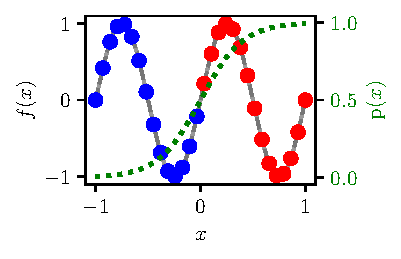
\includegraphics[width=\textwidth]{figures/sota_2/gp_realizations_demo.pdf}
        \caption{Training data clustered into two clusters. The green line represents the classifier probability of belonging to $x > 0$ for $\gamma = 5$.}
        \label{fig:sota_2:sine_1}
    \end{subfigure}\hfill
    \begin{subfigure}[t]{0.48\textwidth}
        \centering
        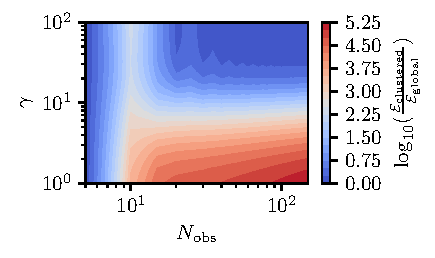
\includegraphics[width=\textwidth]{figures/sota_2/error_fraction_heatmap.pdf}
        \caption{Ratio between the error of the piecewise surrogate model and the error of a global surrogate model as a function of $N_{\mathrm{obs}}$ and $\gamma$.}
        \label{fig:sota_2:sine_2}
    \end{subfigure}
    \caption{Results of the numerical experiment on the sine function.}
    \label{fig:sota_2:sine}
\end{figure}

Fig.~\ref{fig:sota_2:sine} shows the results of this numerical experiment. In Fig.~\ref{fig:sota_2:sine_1} we can see the training data clustered into two clusters, and the classifier probability of belonging to $x > 0$ for $\gamma = 5$, which is a particularly uncertain classifier. In Fig.~\ref{fig:sota_2:sine_2} we can see the ratio between the \gls{mse} of the local surrogate model (using the soft reconstruction in Eq.~\eqref{eq:sota_2:soft_reconstruction}) and the \gls{mse} of a global surrogate model as a function of the number of training points $N_{\mathrm{obs}}$ and the steepness parameter $\gamma$. For large $N_{\mathrm{obs}}$, we can see two interesting behaviors. First, for a very uncertain classifier (small $\gamma$), the error of the piecewise surrogate model is significantly higher than the error of the global surrogate model. This is expected because the soft prediction in Eq.~\eqref{eq:sota_2:soft_reconstruction} is a combination of the predictions of the two local surrogate models, one of which is extrapolating (possibly wrong mean and high variance). For a sharp classifier (large $\gamma$), the error of the piecewise surrogate model is comparable to the error of the global surrogate model, as the soft reconstruction tends to the piecewise one.

\smallskip
\red{The above example suggests that over-clustering does not affect the predictive performances of the surrogate model provided that one either trains a sharp classifier or uses a piecewise reconstruction. If the uncertainty of the classifier is taken into account, introducing a \textit{fake} discontinuity is detrimental to the behavior of the predictive error in its vicinity.}


\section{Score Functions for Local Regressors}
\label{sc:score_functions}

In this section we finally derive the expressions for the score functions $S(\tilde{f}_l, \data_l)$ and the change in global score $\Delta S (l \rightarrow l^{\prime}; \bx_i, \mathbf{z}, \boldsymbol{\beta})$ for both \glspl{gp} and \glspl{pce}. We show that these quantities can be efficiently computed using closed-form formulas, without the need to retrain the local regressors for each membership update, which is crucial for the computational efficiency of our approach.

\subsection{Gaussian Process Models}
\label{sc:gp_models}

A \gls{gp} model represents a response $f(\bx)$ as a series expansion over a set of basis functions,

\begin{equation}
  \tilde{f}(\bx; \boldsymbol{\beta}) = \mathrm{m}_{\boldsymbol{\beta}}(\bx) + \mathrm{k}_{\boldsymbol{\beta}}(\bx, \mathbf{X})^{\top} \mathbf{w}_{\boldsymbol{\beta}} \;,
\end{equation}

where $\mathrm{m}_{\boldsymbol{\beta}}(\bx)$ is the mean function, $\mathrm{k}_{\boldsymbol{\beta}}(\bx, \mathbf{X})$ is the covariance function evaluated at $\bx$ and the training points $\mathbf{X}$, and $\mathbf{w}_{\boldsymbol{\beta}} = (\mathbf{K}_{\boldsymbol{\beta}} + \sigma_n^2 \mathbf{I})^{-1} (\mathbf{y} - \mathbf{m}_{\boldsymbol{\beta}})$ are the weights of the basis functions, with $\mathbf{K}_{\boldsymbol{\beta}}$ being the covariance matrix evaluated at the training points and $\mathbf{m}_{\boldsymbol{\beta}}$ being the mean function evaluated at the training points, see \S\ref{sec:ntools:gpr} for more details. The term $\sigma_n^2$ is a noise term added to the diagonal of the covariance matrix for numerical stability, and is also known as Tikhonov regularization. The hyperparameters $\boldsymbol{\beta}$ of the \gls{gp} model are the parameters that specify the mean and covariance functions, such as the length-scales and the signal variance of the covariance function, and the parameters of the mean function.

\smallskip
As previously stated, a \gls{gp} model is an interpolatory model, i.e., it interpolates the training data, the coefficients are fixed and one needs to fine-tune the hyperparameters $\boldsymbol{\beta}$ to obtain a good fit to the data. A very popular choice for the score function to be maximized during model selection is the log-marginal likelihood of the observations given the hyperparameters, i.e.,

\begin{equation}
  S(\boldsymbol{\beta},\data) = -\frac{1}{2} (\mathbf{y}-\mathbf{m}_{\boldsymbol{\beta}})^{\top} (\mathbf{K}_{\boldsymbol{\beta}} + \sigma_n^2 \mathbf{I})^{-1} (\mathbf{y}-\mathbf{m}_{\boldsymbol{\beta}}) - \frac{1}{2} \log \det (\mathbf{K}_{\boldsymbol{\beta}} + \sigma_n^2 \mathbf{I}) \;.
  \label{eq:clustering:gp_score}
\end{equation}

Other popular choices for the score function include the \gls{loo} predictive probability of the observations, which is not considered in this work, but would entail a similar derivation as the one we are about to present here.

\smallskip
To derive the change in global score $\Delta S (l \rightarrow l^{\prime}; \bx_i)$ when changing the membership of an observation $i$ from its current cluster $l$ to another cluster $l^\prime$, we start by substituting the expression for the score function defined in Eq.~\eqref{eq:clustering:gp_score} into Eq.~\eqref{eq:clustering:change_score}, leading to,

\begin{equation}
  \left.
\begin{aligned}
  \Delta S (l \rightarrow l^{\prime}; \bx_i) &= [\log \p{\data_{l}/ \{\mathbf{d}_i\} \mid \boldsymbol{\beta}_l} - \log \p{\data_{l}\mid \boldsymbol{\beta}_l}]\\
  & \red{+} [\log \p{\data_{l^\prime} \cup \{\mathbf{d}_i\} \mid \boldsymbol{\beta}_{l^\prime}}-\log \p{\data_{l^\prime}\mid \boldsymbol{\beta}_{l^\prime}}]\;.
\end{aligned}
  \right.
  \label{eq:clustering:delta_score}
\end{equation}

The first term corresponds to the change of the log-likelihood of the cluster $z_i$ when removing the $i$-th observation, while the second term corresponds to the change of the log-likelihood of the cluster $l$ when adding the $i$-th observation. To further simplify the expression, we use the rule of conditional probabilities,

\begin{equation}
  \left. 
  \begin{aligned}
    \log \p{\data_{l}/ \{\mathbf{d}_i\} \mid \boldsymbol{\beta}_l} &= \log \p{\data_{l} \mid \boldsymbol{\beta}_l} - \log \p{\mathbf{d}_i \mid \data_{l}/\{\mathbf{d}_i\}, \boldsymbol{\beta}_l} \;,\\
    \log \p{\data_{l^\prime} \cup \{\mathbf{d}_i\} \mid \boldsymbol{\beta}_{l^\prime}} &= \log \p{\data_{l^\prime} \mid \boldsymbol{\beta}_{l^\prime}} + \log \p{\mathbf{d}_i \mid \data_{l^\prime}, \boldsymbol{\beta}_{l^\prime}} \;.
  \end{aligned}
  \right.
  \label{eq:clustering:delta_score_2}
\end{equation}

Substituting Eq.~\eqref{eq:clustering:delta_score_2} into Eq.~\eqref{eq:clustering:delta_score}, we obtain the final expression for the change of the global score,

\begin{equation}
  \Delta S (l \rightarrow l^{\prime}; \bx_i) = - \log \p{\mathbf{d}_i \mid \data_{l}/\{\mathbf{d}_i\}, \boldsymbol{\beta}_l} + \log \p{\mathbf{d}_i \mid \data_{l^\prime}, \boldsymbol{\beta}_{l^\prime}} \;.
  \label{eq:clustering:delta_score_final}
\end{equation}

The first term is the \gls{loo} predictive probability of the observation $i$ using the \gls{gp} model of cluster $l$, while the second term is the predictive probability of the observation $i$ using the \gls{gp} model of cluster $l^\prime$. Both quantities can be cheaply computed without the need to recompute the inverse of the covariance matrix~\cite{gp_rasmussen}.

\subsection{Polynomial Expansions}
\label{sc:pc_expansions}

A polynomial representation of a function $f$ is expressed as a series expansion over a set of multivariate polynomial basis functions,

\begin{equation}
  \tilde{f}(\bx; \boldsymbol{\beta}) = \boldsymbol{\phi}(\bx)^{\top} \boldsymbol{\beta}\;.
\end{equation}

The basis functions $\boldsymbol{\phi}(\bx)$ are typically chosen to be orthogonal polynomials with respect to a certain measure, such as Legendre polynomials for uniform distributions or Hermite polynomials for Gaussian distributions. 

\smallskip
A popular way to fit a polynomial model to data is to use ordinary least squares regression, which corresponds to maximizing the negative \gls{mse} of the observations given the hyperparameters, i.e.,

\begin{equation}
  S(\boldsymbol{\beta}, \data) = \left\|\mathbf{y}- \boldsymbol{\phi}(\mathbf{X})^{\top} \boldsymbol{\beta} \right\|^2 + R(\boldsymbol{\beta}) \;,
  \label{eq:clustering:pc_score}
\end{equation}

where $R(\boldsymbol{\beta})$ is a regularization term that can be added to prevent overfitting. If no regularization is used, the optimal coefficients $\boldsymbol{\beta}$ can be computed in closed-form as $\boldsymbol{\beta} = (\boldsymbol{\phi}(\mathbf{X})^{\top} \boldsymbol{\phi}(\mathbf{X}))^{-1} \boldsymbol{\phi}(\mathbf{X})^{\top} \mathbf{y}$, while if a Tikhonov regularization is used, the optimal coefficients can be computed as $\boldsymbol{\beta} = (\boldsymbol{\phi}(\mathbf{X})^{\top} \boldsymbol{\phi}(\mathbf{X}) + \lambda \mathbf{I})^{-1} \boldsymbol{\phi}(\mathbf{X})^{\top} \mathbf{y}$, for some user-defined regularization parameter $\lambda$. The change in global score $\Delta S (l \rightarrow l^{\prime}; \bx_i, \mathbf{z}, \boldsymbol{\beta})$ when changing the membership of an observation $i$ from its current cluster $l$ to another cluster $l^\prime$ can be derived by substituting the expression for the score function defined in Eq.~\eqref{eq:clustering:pc_score} into Eq.~\eqref{eq:clustering:change_score}, leading to,

\begin{equation}
  \Delta S (l \rightarrow l^{\prime}; \bx_i) = - (y_i - \tilde{f}_{l^\prime}(\bx_i; \boldsymbol{\beta}_{l^\prime}))^2 + (y_i - \tilde{f}_{l}(\bx_i; \boldsymbol{\beta}_{l}))^2 \;.
  \label{eq:clustering:delta_score_pc}
\end{equation}

In Eq.~\eqref{eq:clustering:delta_score_pc} the first term is the negative squared error of the observation $i$ using the polynomial model of cluster $l^\prime$, while the second term is the negative squared error of the observation $i$ using the polynomial model of cluster $l$. Effectively, the change in global score evaluates how well the observation $i$ is predicted by the model of cluster $l^\prime$ compared to how well it was predicted by the model of cluster $l$. 

\smallskip
Notice that, contrary to the case of \glspl{gp}, this quantity holds also when multiple points change their membership at the same time.

\section{Example 1: Discontinuous Function}
\label{sc:tc_1}

In this section, we apply the clustering algorithm to an analytical function defined on the hypercube $[-1,1]^d$. The function is designed to have both zeroth and first-order discontinuities, which makes it a challenging test case for surrogate modeling. We define the function $f$ by partitioning the input space into three subdomains $\Omega_1$, $\Omega_2$, and $\Omega_3$ as follows,

\begin{equation}
  \left. 
    \begin{aligned}
      &\Omega_1 = \{ \bx \in [-1,1]^d\, :\, \lVert\bx\rVert_2 < R(d)\} \,\\
      &\Omega_2 = \{ \bx \in [-1,1]^d\, :\, \sum_{i=1}^{d} x_i < 0\,\text{and}\, \lVert\bx\rVert_2 > R(d)\} \,\\
      &\Omega_3 = \{ \bx \in [-1,1]^d\, :\, \sum_{i=1}^{d} x_i \geq 0\,\text{and}\, \lVert\bx\rVert_2 > R(d)\} .
    \end{aligned}
  \right.
  \label{eq:clustering:sudomains}
\end{equation}

We numerically estimate $R(d)$ such that each subdomain $\Omega_k$ occupies one third of the volume of $[-1,1]^d$. The function $f$ is then defined as follows,

\begin{equation}
  f(\bx) =
  \left\{
    \begin{aligned}
      & 1-\exp\!\left(\lVert\bx\rVert_2^2 - R^2(d)\right) &\text{if } \bx \in \Omega_1 \,\\
      &0.1\,\left( \lVert\bx\rVert_2^2 - R^2(d) \right) &\text{if } \bx \in \Omega_2 \,\\
      &-0.1\,\left( \lVert\bx\rVert_2^2 - R^2(d) \right) &\text{if } \bx \in \Omega_3 \,.
    \end{aligned}
  \right.
  \label{eq:clustering:example}
\end{equation}

{
\begin{figure}[htbp]
  \begin{subfigure}{0.49\linewidth}
    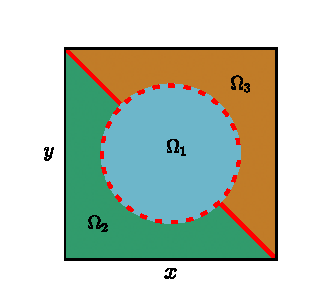
\includegraphics[width=1.0\textwidth]{figures/clustering/partition_plot.pdf}
    \caption{Partition of the domain in 2D.}
  \end{subfigure}
  \begin{subfigure}{0.49\linewidth}
    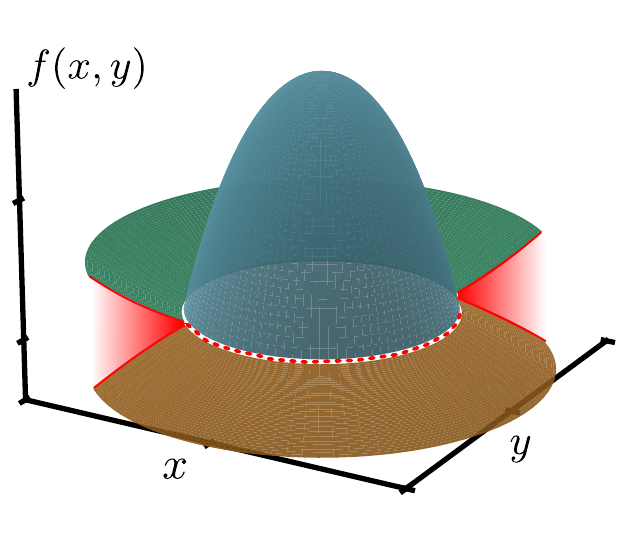
\includegraphics[width=1.0\textwidth]{figures/clustering/function_plot_compressed.png}
    \caption{2D function plot.}
  \end{subfigure}
  \caption{Partition of the domain (left) and 2D function plot (right) of the function $f$ defined in Eq.~\eqref{eq:clustering:example}. The different colors correspond to the different smooth subdomains of the input space. Continuous red lines indicate first order discontinuities, while dashed red lines indicate jumps.}
  \label{fig:clustering:example}
\end{figure}
}

Fig.~\ref{fig:clustering:example} depicts Eq.~\eqref{eq:clustering:example} in 2D. The interface between $\Omega_2$ and $\Omega_3$ has a jump, whereas the boundary of $\Omega_1$ has a jump in the gradient. \red{Approximating Eq.~\eqref{eq:clustering:example} with a single global surrogate (e.g., \gls{gp} or \gls{pce}) is severely hindered by these zeroth and first-order discontinuities. Additionally, because the subdomains in Eq.~\eqref{eq:clustering:sudomains} are not necessarily convex, classical clustering algorithms struggle to partition them effectively.}


\smallskip
\red{Unless otherwise specified, all subsequent tests are performed using \glspl{gp} with a constant mean and an \gls{rbf} covariance function, whose hyperparameters are tuned by \gls{mle} as described in \S\ref{sec:ntools:gpr:mml}. These are paired with a \gls{svm} with an \gls{rbf} kernel, whose hyperparameters are trained using the span minimization procedure detailed in \S\ref{sec:ntools:svm:hyperparameter}. Algorithm~\ref{alg:clustering:model_clustering} is initialized with a temperature of $T^{(0)}=1$ and a decay rate of $\alpha_T = 0.99$. It allows updates of up to $20\%\,\nobs$ per iteration, enforces a minimum cluster size of $10$ points alongside a confusion threshold of $0.5$, and terminates when the relative change in the global score remains below $1\%$ for three consecutive iterations.}

\smallskip
\red{The initial partitioning is either computed using a K-means algorithm (on the $\bx$ coordinates only), see Alg.~\ref{alg:kmean} for the implementation details, or a \gls{dp}-\gls{gmm}~\cite{Sudret2023} clustering scheme. For the latter, we employ an empirical Normal-Inverse-Wishart prior scaled for $6$ expected clusters with a prior precision of $0.1$ and $d+2$ degrees of freedom, alongside a $\mathrm{Gamma}(1,1)$ prior for the concentration parameter.}


\subsection{Robustness: Choosing the Initial Partition}
\label{sc:K0}

In this subsection we numerically investigate the robustness of the clustering algorithm with respect to the choice of the initial \red{clustering of the training data}. We test the stochastic optimization scheme starting from an initial K-means clustering of the training data with $L^{(0)}=3$, $L^{(0)}=40$. We then test the deterministic optimization scheme (i.e. $T=0$) with an initial clustering computed using a \gls{dp}-\gls{gmm}. 


\begin{figure}[htbp]
  \centering%
  \begin{subfigure}[b]{0.49\linewidth}
    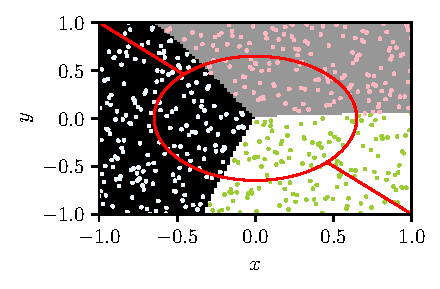
\includegraphics[width=1.0\textwidth]{figures/clustering/cluster_0_3.pdf}
    \caption{Initial clustering for $L^{(0)}=3$.}
  \end{subfigure}%
  \hfill%
  \begin{subfigure}[b]{0.49\linewidth}
    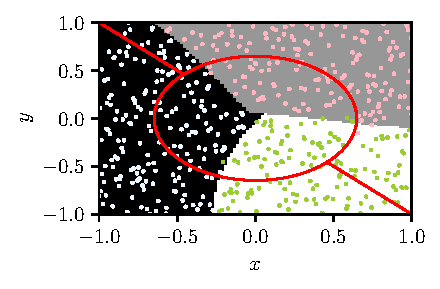
\includegraphics[width=1.0\textwidth]{figures/clustering/cluster_final_3.pdf}
    \caption{Final clustering for $L^{(0)}=3$.}
  \end{subfigure}
  
  \vspace{1em}
  
  \begin{subfigure}[b]{0.49\linewidth}
    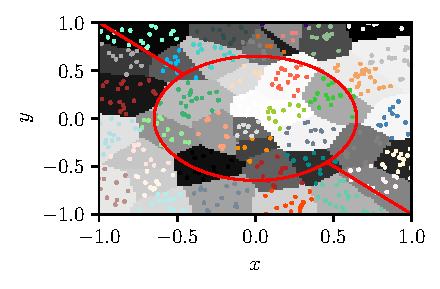
\includegraphics[width=1.0\textwidth]{figures/clustering/cluster_0_40.pdf}
    \caption{Initial clustering for $L^{(0)}=40$.}
  \end{subfigure}%
  \hfill%
  \begin{subfigure}[b]{0.49\linewidth}
    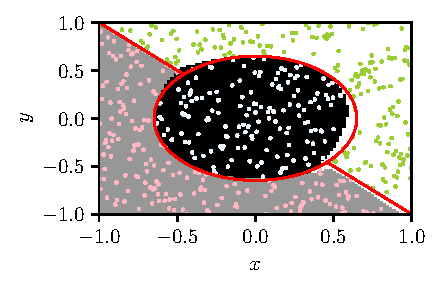
\includegraphics[width=1.0\textwidth]{figures/clustering/cluster_final_40.pdf}
    \caption{Final clustering for $L^{(0)}=40$.}
  \end{subfigure}
  
  \vspace{1em}
  
  \begin{subfigure}[b]{0.49\linewidth}
    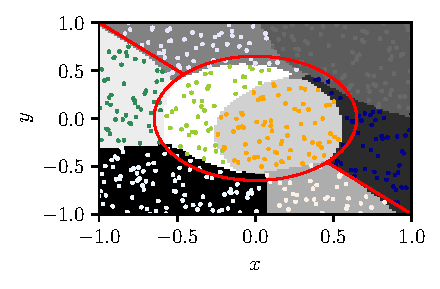
\includegraphics[width=1.0\textwidth]{figures/clustering/cluster_0_dpmm.pdf}
    \caption{Initial clustering computed using \gls{dp}-\gls{gmm}.}
  \end{subfigure}%
  \hfill%
  \begin{subfigure}[b]{0.49\linewidth}
    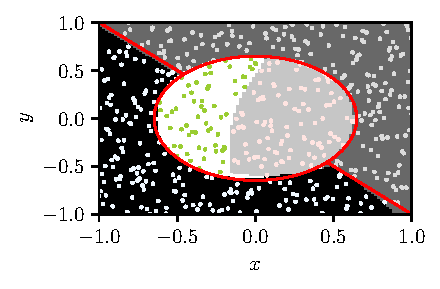
\includegraphics[width=1.0\textwidth]{figures/clustering/cluster_final_dpmm.pdf}
    \caption{Final clustering for \gls{dp}-\gls{gmm}.}
  \end{subfigure}
  
  \caption{The clustering algorithm for different initial number of clusters $L^{(0)}$. Red lines indicate discontinuities of the function, points are colored according to their cluster membership and shaded areas represent the identified subdomains.}
  \label{fig:clustering:L0}
\end{figure}

In Fig.~\ref{fig:clustering:L0}, we show the  final cluster distribution for different initial number of clusters $L^{(0)}$. The top row corresponds to the case $L^{(0)}=3$, which is equal to the actual number of smooth subdomains. Such initial clustering is not rich enough to capture the structure of the function, and the algorithm is not able to make any meaningful improvement, leading to a poor final clustering. 

\smallskip
In the middle row, we set $L^{(0)}=40$, which is higher than the actual number of smooth subdomains. The initial clustering is rich enough to capture the structure of the function, and the algorithm is able to effectively explore the search space and yield a good final clustering, with the final number of clusters being \red{equal to the number of subdomains.}

\smallskip
The bottom row corresponds to the case in which the initial clustering is computed using a \gls{dp}-\gls{gmm}. The initial clustering is excellent, with 8 clusters roughly capturing \red{the structure of the smooth subdomains}. However, there are some mis-clustered points, especially around \red{non-convex boundaries}. The deterministic optimization scheme is able to refine the initial clustering and yield a good final clustering, moving the mis-clustered points percentage from $7\%$ to $0\%$ and reducing the number of clusters from $8$ to $4$. 

\begin{figure}[htbp]
  \centering
  
  % --- First Subfigure (a) ---
  \begin{subfigure}[t]{0.5\textwidth}
    \centering
    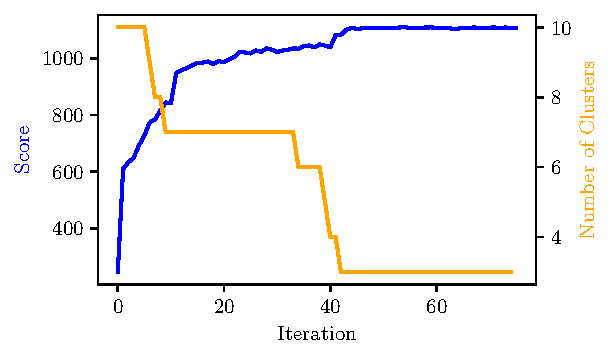
\includegraphics[width=\textwidth]{figures/clustering/scores_clusters.pdf}
    \caption{Global score and cluster count evolution for $T^{(0)}=1$.}
    \label{fig:clustering:score_clusters}
  \end{subfigure}
  \hfill % Adds horizontal space between the two figures
  % --- Second Subfigure (b) ---
  \begin{subfigure}[t]{0.48\textwidth}
    \centering
    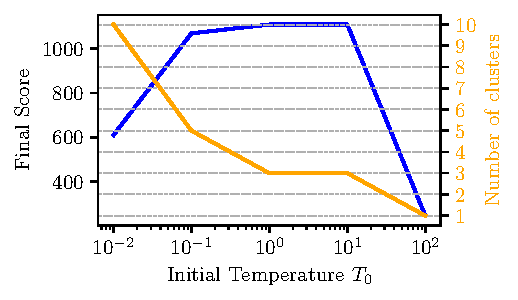
\includegraphics[width=\textwidth]{figures/clustering/grid_search.pdf}
    \caption{\red{Grid-search over the initial temperature.}}
    \label{fig:clustering:gsearch}
  \end{subfigure}
  
  % --- Main Caption ---
  \caption{Analysis of the global score and cluster count in $d=2$ for $500$ points and initial K-means clustering with $L^{(0)}=10$.}
  \label{fig:clustering:combined_analysis}
\end{figure}

\red{Finally, in Fig.~\ref{fig:clustering:combined_analysis}, we report a detailed view of the global score and cluster count for $d=2$ with $500$ observations and an initial K-means partition of $L^{(0)}=10$. In Fig.~\ref{fig:clustering:score_clusters}, we show how these metrics evolve over the algorithm's iterations for a fixed initial temperature of $T^{(0)}=1$. The global score does not increase monotonically, especially in the early stages, a consequence of the stochastic nature of the optimization scheme and the fact that clusters are merged and purged. At the end, when the temperature is low, the global score increases monotonically and reaches a local maximum. In Fig.~\ref{fig:clustering:gsearch}, we show how the final values change if we vary the initial temperature. We see that an initial temperature between $1$ and $10$ yields the highest global score with the lowest number of clusters. A lower initial temperature leads to too many clusters, while a higher one leads to too few clusters, caused by aggressive mixing and merging.}

\subsection{Results: Mis-Clustered Points}

In this section, we investigate the robustness of the clustering algorithm with respect to data scarcity. In particular, we analyze the fraction of mis-clustered points as a function of the number of observations and the dimensionality of the input space, to assess how well the algorithm can identify the discontinuities of the function. All results are averaged over $30$ runs with different \gls{lhs} \gls{ndoe}. \red{We compare the results of Alg.~\ref{alg:clustering:model_clustering} (initialized with $10$ clusters computed using K-means) against a single global \gls{gp} and a \gls{dp}-\gls{gmm} clustering scheme.}

\begin{figure}[htbp]
  \centering
  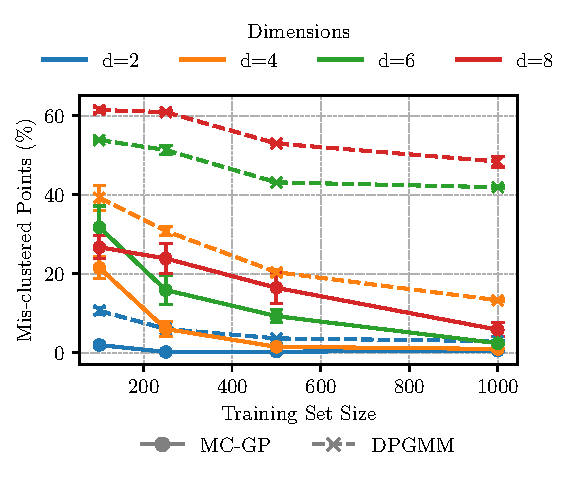
\includegraphics[width=0.7\textwidth]{figures/clustering/outliers.pdf}
  \caption{The percentage of points that overlap with the discontinuities of the function $f$ defined in Eq.~\eqref{eq:clustering:example} as a function of the number of observations and the dimensionality of the input space. MC-GP (Model-Clustering \gls{gp}) stands for Alg.~\ref{alg:clustering:model_clustering}.}
  \label{fig:clustering:outliers}
\end{figure}


\smallskip
Fig.~\ref{fig:clustering:outliers} shows the fraction of mis-clustered points versus training-set size and dimension. \blue{To evaluate this error metric, we map each discovered cluster $\data_l$ to a \textit{reference subdomain}, defined as the underlying subdomain from Eq.~\eqref{eq:clustering:sudomains} that contributes the majority of the points to $\data_l$. Any points within $\mathcal{O}_l$ that belong to this reference subdomain are deemed correctly clustered, whereas all other points in the cluster are counted as mis-clustered, here denoted with $\mathcal{O}_l^{\text{mis}}$. The percentage of mis-clustered points is then calculated as the ratio of mis-clustered points to the total number of points,}

\begin{equation}
  \mathcal{E}_{\mathrm{clus.}} = \dfrac{1}{\nobs}\summ{i}{1}{l} |\mathcal{O}_l^{\text{mis}}| \;.
\end{equation}

The results show that the fraction of mis-clustered points decreases as the number of observations increases, confirming that data scarcity is a major factor in mis-clustering. \red{The results also show that our model clustering scheme is more robust than a \gls{dp}-\gls{gmm} clustering scheme, which severely underperforms in high dimensions.}

Increasing the dimensionality of the input space leads to a higher fraction of mis-clustered points, especially for small training sets. The percentage improves as the training set grows. \red{The results of our model clustering scheme are more robust than the ones of a \gls{dp}-\gls{gmm} clustering scheme.}

\smallskip
\red{Concering our clustering scheme, }we attribute mis-clustering primarily to data scarcity rather than to algorithmic failure (e.g., convergence to a poor local optimum): in high dimensions and few data points, the global score does not correlate well with the quality of the clustering. We test this hypothesis by initializing the clustering algorithm with the exact partition of the input space, Eq.~\eqref{eq:clustering:sudomains}, and then running it in the deterministic regime (i.e., $T=0$) to see whether the exact partitioning corresponds to a maximum of the global score. We repeat this experiment 30 times with different \gls{lhs}-\gls{ndoe} for $d=6$ and $100$ and $500$ observations. We also compute the \gls{mse} on an independent \gls{lhs}-\gls{ndoe} of $100'000$ points.

{
\begin{figure}[htbp]
  \begin{subfigure}{0.49\linewidth}
    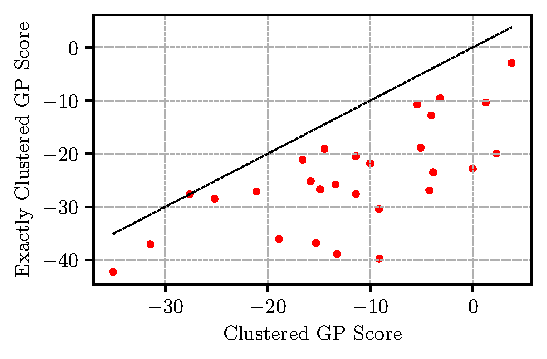
\includegraphics[width=1.0\textwidth]{figures/clustering/test_scores_scatter_100pt.pdf}
    \caption{Global score, grid of 100 points.}
  \end{subfigure}
  \begin{subfigure}{0.49\linewidth}
    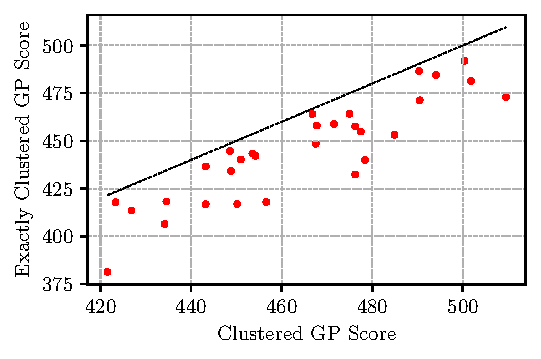
\includegraphics[width=1.0\textwidth]{figures/clustering/test_scores_scatter_500pt.pdf}
    \caption{Global score, grid of 500 points.}
  \end{subfigure}
  \begin{subfigure}{0.49\linewidth}
    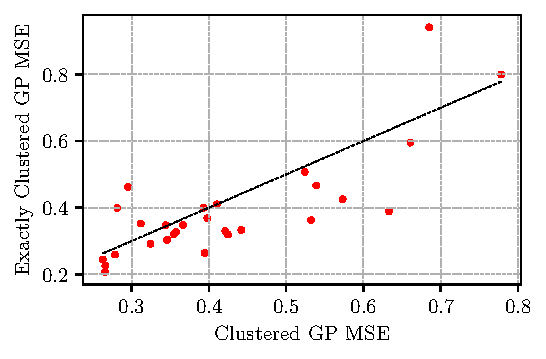
\includegraphics[width=1.0\textwidth]{figures/clustering/test_scores_mse_scatter_100pt.pdf}
    \caption{Average \gls{mse}, grid of 100 points.}
  \end{subfigure}
  \begin{subfigure}{0.49\linewidth}
    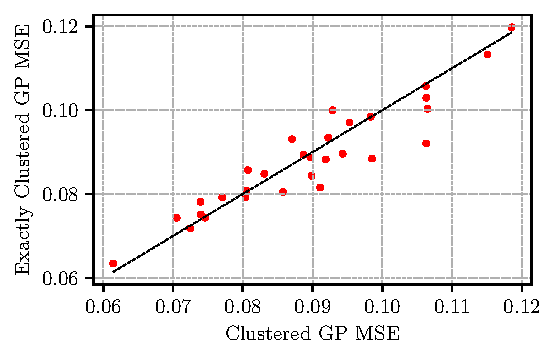
\includegraphics[width=1.0\textwidth]{figures/clustering/test_scores_mse_scatter_500pt.pdf}
    \caption{Average \gls{mse}, grid of 500 points.}
  \end{subfigure}
  \caption{Global score (top) and average \gls{mse} (bottom) for the exactly clustered model and the final model obtained using the clustering algorithm. The dimensionality of the input space is $6$ while the number of observations is $100$ (left) and $500$ (right). Each point corresponds to a different training grid design.}
  \label{fig:clustering:test_outliers}
\end{figure}
}

In Fig.~\ref{fig:clustering:test_outliers}, the vertical axis reports the score (or \gls{mse}) of the initial, exactly partitioned configuration, whereas the horizontal axis reports the same quantity for the final configuration obtained by running the clustering algorithm. Results show that the global score consistently increases from the initial to the final configuration, confirming that the algorithm faithfully maximizes $S_{\mathrm{global}}$; the reason mis-clustering persists at low $\nobs$ is that $S_{\mathrm{global}}$ itself is a poor proxy for clustering quality in that regime, not that the optimizer fails. Furthermore, we see that for $100$ observations, the final \gls{mse} is mostly worse than the initial \gls{mse}, while for $500$ observations, there are no visible differences. Overall this analysis confirms that the global score is not a good proxy for the quality of the clustering when data is scarce, but becomes more reliable as the training set grows, which explains the improvement in mis-clustering with more data.

{
\begin{figure}[htbp]
  \begin{subfigure}{0.49\linewidth}
    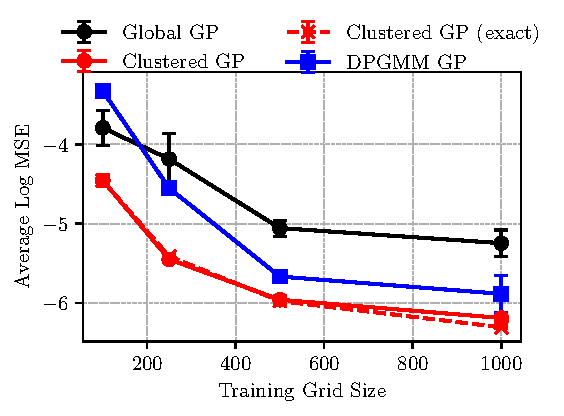
\includegraphics[width=1.0\textwidth]{figures/clustering/test_scores_dim=2.0.pdf}
    \caption{Average log \gls{mse}, dimension 2.}
  \end{subfigure}
  \begin{subfigure}{0.49\linewidth}
    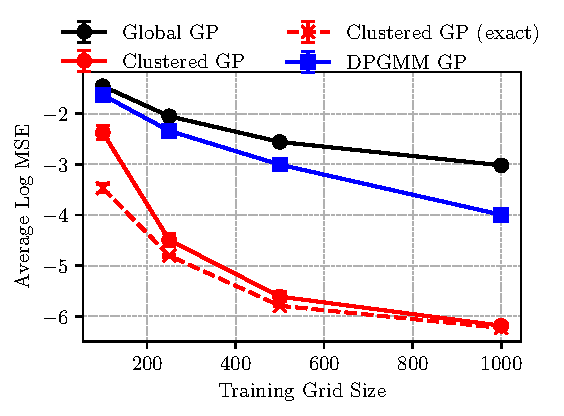
\includegraphics[width=1.0\textwidth]{figures/clustering/test_scores_dim=4.0.pdf}
    \caption{Average log \gls{mse}, dimension 4.}
  \end{subfigure}
  \begin{subfigure}{0.49\linewidth}
    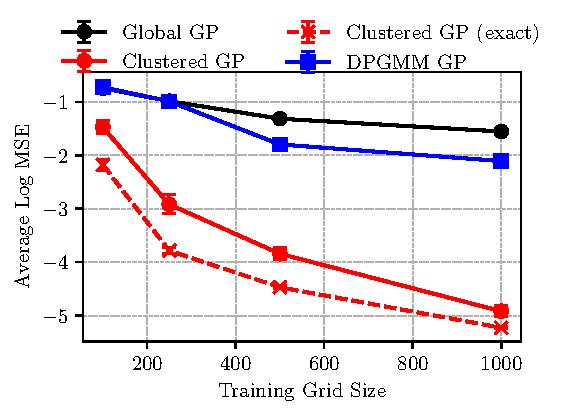
\includegraphics[width=1.0\textwidth]{figures/clustering/test_scores_dim=6.0.pdf}
    \caption{Average log \gls{mse}, dimension 6.}
  \end{subfigure}
  \begin{subfigure}{0.49\linewidth}
    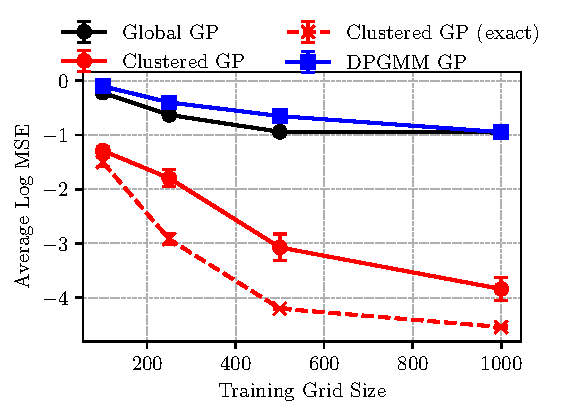
\includegraphics[width=1.0\textwidth]{figures/clustering/test_scores_dim=8.0.pdf}
    \caption{Average log \gls{mse}, dimension 8.}
  \end{subfigure}
  \caption{Average log \gls{mse} for the global \gls{gp} and the smooth reconstruction using the clustered \gls{gp}, a \gls{dp}-\gls{gmm}, and the exactly clustered \gls{gp} as a function of the number of observations and the dimensionality of the input space.}
  \label{fig:clustering:mse_dim_test}
\end{figure}
}

Fig.~\ref{fig:clustering:mse_dim_test} completes the analysis by showing the average log-\gls{mse} on the test \gls{ndoe} for variable design sizes and dimensions. The figure compares the \gls{mse} of a single global \gls{gp} and the \gls{mse} of the piecewise \gls{gp} using the smooth reconstruction. For the latter, we compare the exactly clustered model (i.e., clustering obtained from Eq.~\eqref{eq:clustering:sudomains}) and the final model obtained using the clustering algorithm (initial partition and settings as the ones for Fig.~\ref{fig:clustering:outliers}) \red{and a \gls{dp}-\gls{gmm} clustering scheme}. We see that the exactly clustered \gls{gp} consistently outperforms all other models but our algorithm performs almost as well as the exactly clustered one, especially as we increase the number of observations. Even in data-scarce regimes, the piecewise \gls{gp} obtained using the clustering algorithm outperforms the global \gls{gp} \red{and a simple \gls{dp}-\gls{gmm} clustering scheme}.

\smallskip
\red{In particular, the \gls{dp}-\gls{gmm} clustering scheme proposed by~\cite{Sudret2023} is not able to understand the structure of the function in high dimensions, leading to a poor performance of the piecewise \gls{gp} model. We attribute this to the fact that the \gls{dp}-\gls{gmm} clustering scheme struggles to capture the non-convexity of the smooth subdomains, which is instead captured by our clustering algorithm.}

\subsection{Results: Global Reconstruction}

In this section, we analyze the different approaches for the global reconstruction of the function $f$ and the smooth subdomains identified by the clustering algorithm. 

{
\begin{figure}[htbp]
  \begin{subfigure}{0.49\linewidth}
    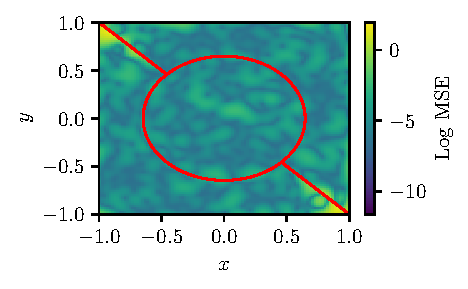
\includegraphics[width=1.0\textwidth]{figures/clustering/errors_global.pdf}
    \caption{Global \gls{gp}.}
  \end{subfigure}
  \hfill
  \begin{subfigure}{0.49\linewidth}
    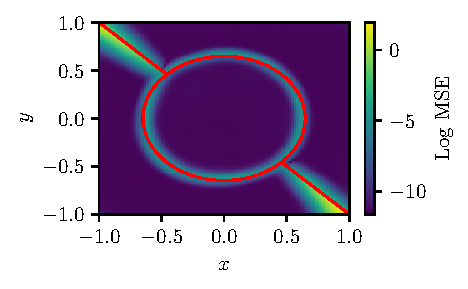
\includegraphics[width=1.0\textwidth]{figures/clustering/errors_smooth.pdf}
    \caption{Clustered \gls{gp}, smooth reconstruction.}
  \end{subfigure}
  \hfill
  \begin{subfigure}{0.49\linewidth}
    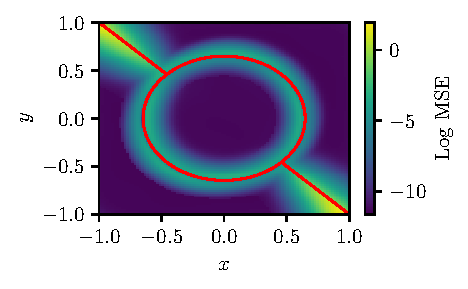
\includegraphics[width=1.0\textwidth]{figures/clustering/errors_gmm.pdf}
    \caption{Clustered \gls{gp}, \gls{gmm} reconstruction.}
  \end{subfigure}
  \hfill
  \begin{subfigure}{0.49\linewidth}
    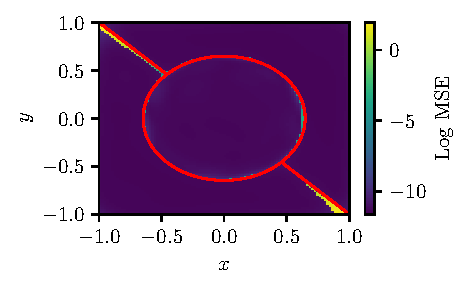
\includegraphics[width=1.0\textwidth]{figures/clustering/errors_hard.pdf}
    \caption{Clustered \gls{gp}, piecewise reconstruction.}
  \end{subfigure}
  \caption{Reconstruction errors for the different \gls{gp} models in the domain $\Omega$.}
  \label{fig:clustering:error_domain}
\end{figure}
}


Fig.~\ref{fig:clustering:error_domain} illustrates the behavior of the \gls{mse} on the 2D domain $\Omega$ for the different \gls{gp} models. The most capturing difference is between global and clustered \glspl{gp}: the presence of discontinuities leads to a high \gls{mse} everywhere in the domain for the global \gls{gp}, as such discontinuities poison the behavior of the model even in smooth regions. The clustered \gls{gp}, on the contrary, has a much lower \gls{mse} in the smooth subdomains, with the highest errors concentrated around boundaries. The high \gls{mse} around boundaries is due to increased uncertainty of the model in these regions, either caused by an extrapolatory behavior of the model (for the smooth reconstruction) or by the additional model uncertainty (for the \gls{gmm} reconstruction). The piecewise reconstruction seems to be least affected as it does not include the domain uncertainty but it is also the one with the highest \gls{mse} around boundaries, as it does not include any uncertainty and thus is more affected by mis-classification of points around jumps.


\begin{figure}[htbp]
  \begin{subfigure}[t]{0.49\linewidth}
    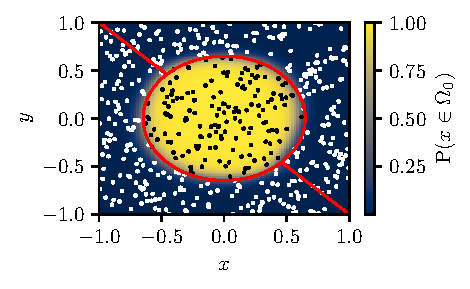
\includegraphics[width=1.0\textwidth]{figures/clustering/p0.pdf}
    \caption{\glspl{svc} probability for the cluster $k=0$.}
  \end{subfigure}
  \begin{subfigure}[t]{0.49\linewidth}
    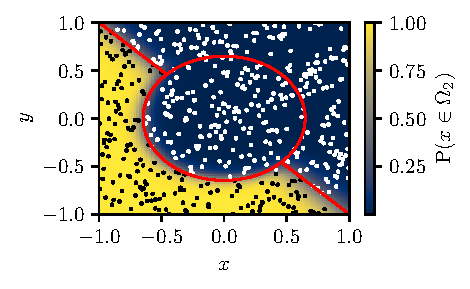
\includegraphics[width=1.0\textwidth]{figures/clustering/p2.pdf}
    \caption{\glspl{svc} probability for the cluster $k=1$.}
  \end{subfigure}
  \caption{The \glspl{svc} probabilities for the clusters $k=0$ (left) and $k=1$ (right). The red lines correspond to the curves in which the function is not differentiable.}
  \label{fig:clustering:svc_probs}
\end{figure}

Fig.~\ref{fig:clustering:svc_probs} illustrates the soft reconstruction of the partition of $\Omega$ via \glspl{svc} probabilities. Black points denote points assigned to the displayed cluster, whereas white points denote points assigned elsewhere. Notice that points near the boundaries have intermediate probabilities, reflecting the model's uncertainty in these regions. These are the points that can actually change their cluster membership during the optimization process.

\subsection{Results: Polynomial Expansion}
As a proof of concept, we also apply the clustering algorithm with polynomial expansions as local regressors. The complex structure of the function $f$, defined in Eq.~\eqref{eq:clustering:example}, motivates the use of a clustering approach, as a single global polynomial would struggle to capture the behavior of $f$ across the entire domain. We use a polynomial expansion of total degree $2$ with Hermite basis functions. Polynomials are trained by minimum \gls{mse} regression, and the change in global score is computed using Eq.~\eqref{eq:clustering:delta_score_pc}. The initial clustering corresponds to a K-means clustering on the $\bx$ coordinates with $L^{(0)}=10$. We perform a stochastic optimization with a fixed initial temperature $T^{(0)}=1$.

\begin{figure}[htbp]
  \begin{subfigure}{0.49\linewidth}
    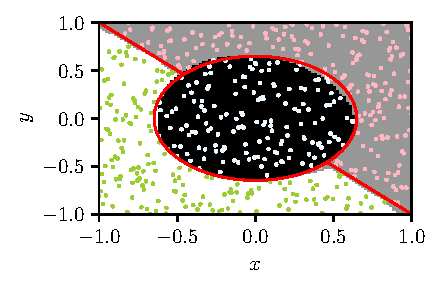
\includegraphics[width=1.0\textwidth]{figures/clustering/cluster_final_poly.pdf}
    \caption{Final clustering for the polynomial expansion. Points are colored according to the cluster they belong to. The red line indicates discontinuities of the function.}
  \end{subfigure}
  \begin{subfigure}{0.49\linewidth}
    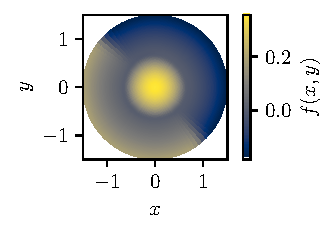
\includegraphics[width=1.0\textwidth]{figures/clustering/prediction_tc1_poly.pdf}
    \caption{Smooth reconstruction of the function $f$ using the clustered polynomial expansion.}
  \end{subfigure}
  \caption{The final clustering (left) and the smooth reconstruction (right) for the polynomial expansion. The red lines correspond to the curves in which the function is not differentiable.}
  \label{fig:clustering:poly_expansion_tc1}
\end{figure}

In Fig.~\ref{fig:clustering:poly_expansion_tc1}, we show the final clustering and the smooth reconstruction of the function $f$ using the clustered polynomial expansion. The algorithm is able to identify the discontinuities of the function and to reconstruct the smooth subdomains effectively. The final number of clusters is $3$, which is equal to the actual number of smooth subdomains.  

\section{Example, Smooth Function with Different Regimes}
\label{sc:tc_2}


In this section, we apply the clustering algorithm to a smooth function defined on the hypercube $[-1,1]^d$. The function is designed to be continuous and differentiable across the entire input space, but to exhibit two different regimes in different regions of the input space with an abrupt transition between them. The goal of this test case is to investigate the performance of the clustering algorithm in a scenario in which the function does not have any discontinuity, but still exhibits a complex structure that may be challenging for a single global surrogate model to capture effectively.

\smallskip
To this end, we generate synthetic data using a cosine function whose amplitude and frequency vary smoothly over the input space, i.e. $[-1,1]^d$:

\begin{equation}
  \left. 
    \begin{aligned}
      &f(\bx) = (1-w(\bx)) A_1 \cos(2 \pi f_1(d)\ ||\bx||_2) + w(\bx) A_2 \cos(2 \pi f_2(d)\ ||\bx||_2) \;.\\
      &w(\bx) = 1/(1+\exp( -\beta(d) (||\bx||_2 - R(d)))) \,.
    \end{aligned}
  \right.
  \label{eq:clustering:function_nonstationary}
\end{equation}

\begin{table}[htbp]
  \centering
  % Use a smaller font and booktabs style (no vertical rules) for cleaner appearance
  \begin{tabular}{|ccccc|}
    \hline
    $A_1$ & $A_2$ & $f_1$ & $f_2$ & $\beta$ \\
    \hline
    1.0 & 0.1 & 1.0 & 5.0 & 10.0 \\
    \hline
  \end{tabular}
  \caption{Base reference parameters ($d=2$) used to generate the synthetic data in Eq.~\eqref{eq:clustering:function_nonstationary}.}
  \label{tab:params_synthetic}
\end{table}

The reference ($d=2$) parameters used to generate the synthetic data are reported in Table~\ref{tab:params_synthetic}. The function $w(\bx)$ is a smooth step function that transitions from $0$ to $1$ around the radius $R(d)$. Similarly to the previous example, the radius $R(d)$ is numerically determined for each dimension $d$ such that the inner region ($||\bx||_2 < R(d)$) and outer shell ($||\bx||_2 > R(d)$) occupy an equal fraction of the volume of $\Omega$. 

\smallskip
As the dimensionality $d$ increases, the geometric size of the hypercube domain expands; the maximum distance from the origin to a corner is $\sqrt{d}$, forcing $R(d)$ to increase accordingly. If the frequencies and transition sharpness were kept constant, higher dimensions would artificially contain more radial oscillations and a proportionally sharper transition boundary, making the underlying regression problem inherently more complex. To guarantee a fair, apples-to-apples evaluation that tames the curse of dimensionality (at least for moderate dimensions $d \leq 8$), the parameters are scaled relative to the 2-dimensional reference case ($R_{ref} \approx 0.798$). Specifically, the inner frequency and the transition sharpness are scaled inversely proportional to the inner domain size ($f_1(d) = f_1 \frac{R_{ref}}{R(d)}$ and $\beta(d) = \beta \frac{R_{ref}}{R(d)}$), while the outer frequency is scaled according to the outer domain size ($f_2(d) = f_2 \frac{\sqrt{2} - R_{ref}}{\sqrt{d} - R(d)}$). This ensures that the total number of wave periods and the proportional width of the transition region remain strictly invariant across all dimensions.

\begin{figure}[htbp]
  \centering
  
  % Top Row: Images only
  \begin{subfigure}[t]{0.48\textwidth}
    \vspace{0pt}
    \centering
    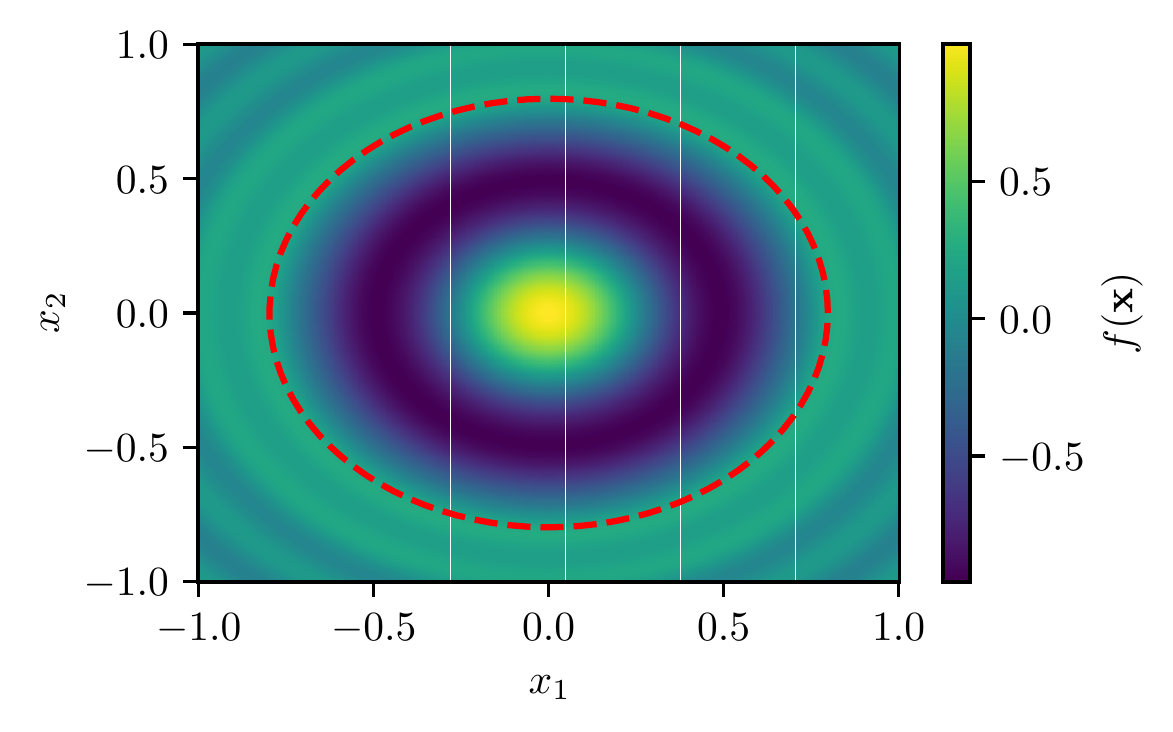
\includegraphics[width=\textwidth]{figures/clustering/function_2d_compressed.png}
  \end{subfigure}
  \hfill
  \begin{subfigure}[t]{0.48\textwidth}
    \vspace{0pt}
    \centering
    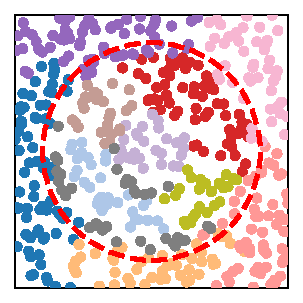
\includegraphics[width=0.6\textwidth]{figures/clustering/plot_sklearn_dpgmm.pdf}
  \end{subfigure}
  
  % Bottom Row: Captions only
  \begin{subfigure}[t]{0.48\textwidth}
    \caption{True function landscape.}
    \label{fig:clustering:function_2d:true}
  \end{subfigure}
  \hfill
  \begin{subfigure}[t]{0.48\textwidth}
    \caption{\gls{dp}-\gls{gmm} clustering in 2D. points are colored according to their assigned cluster.}
    \label{fig:clustering:function_2d:dpgmm}
  \end{subfigure}
  
  \caption{2D function plot of the function $f$ defined in Eq.~\eqref{eq:clustering:function_nonstationary} (left). The dashed red circle indicates the line in which the behavior of the function transitions. On the right, the initial clustering obtained via a \gls{dp}-\gls{gmm}.}
  \label{fig:clustering:function_2d}
\end{figure}

In Fig.~\ref{fig:clustering:function_2d:true}, we show the function $f$ defined in Eq.~\eqref{eq:clustering:function_nonstationary} in 2D. The function smoothly transitions from a low frequency, high amplitude cosine function to a high frequency, low amplitude cosine function around the dashed red circle. Such behavior, coupled with the ring-like structure of the data makes it particularly challenging for a \gls{dp}-\gls{gmm} clustering to be effective. Indeed, in Fig.~\ref{fig:clustering:function_2d:dpgmm} we see the results of such clustering to some $500$ training data-points. Clusters struggle to capture the structure of the subdomains, resulting in multiple disconnected clusters.

\begin{figure}[htbp]
  \centering
  \begin{subfigure}{0.49\linewidth}
    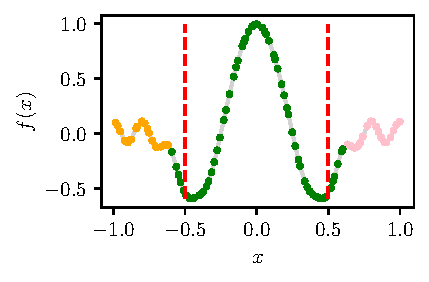
\includegraphics[width=1.0\textwidth]{figures/clustering/clusters_1_100_0.pdf}
    \caption{Final clustering for $d=1$ and $n=100$. Points are colored according to the cluster they belong to. The dashed red line indicates the line in which the behavior of the function transitions.}
  \end{subfigure}
  \begin{subfigure}{0.49\linewidth}
    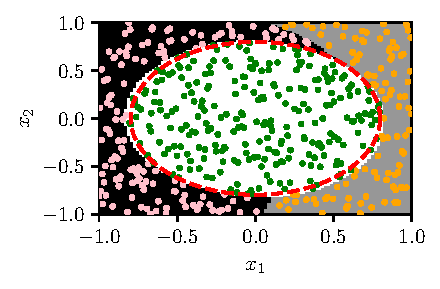
\includegraphics[width=1.0\textwidth]{figures/clustering/clusters_2_500_0.pdf}
    \caption{Final clustering for $d=2$ and $n=500$. Points are colored according to the cluster they belong to. The dashed red line indicates the line in which the behavior of the function transitions. }
  \end{subfigure}
  \caption{The clustering result for the non-stationary function defined in Eq.~\eqref{eq:clustering:function_nonstationary} in 1D (left) and 2D (right).}
  \label{fig:clustering:tc2:mc}
\end{figure}

In Fig.~\ref{fig:clustering:tc2:mc}, we show the clustering result in 1D and 2D. The algorithm was initialized with an initial K-means clustering of size $10$ and a temperature of $1.0$. In both cases, the identified clusters represent the different regimes of the function. Although our algorithm splits the outer region into two clusters, it does not create any disconnected clusters, unlike the \gls{dp}-\gls{gmm} clustering algorithm.

\smallskip
Once clustering, classification and regression are completed, we can investigate the spatial behavior of the hyperparameters of the local \glspl{gp}. We can define a \textit{smooth} reconstruction of the hyperparameters, $\bpsi_{\mathrm{smooth}}(\bx)$, using the \glspl{svc} probabilities and the hyperparameters of the local \glspl{gp}, $\bpsi_l$, as follows,

\begin{equation}
  \bpsi(\bx) = \sum_{l=1}^{L} \mathbb{P}_{\mathrm{SVC}}(l \mid \bx_i, \boldsymbol{\gamma}) \ \bpsi_l \,.
  \label{eq:clustering:smooth_hyper}
\end{equation}

\begin{figure}[htbp]
  \centering
  \begin{subfigure}{0.49\linewidth}
    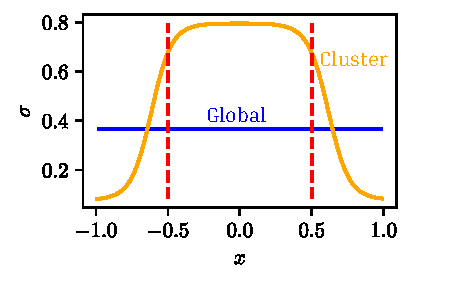
\includegraphics[width=1.0\textwidth]{figures/clustering/params_1_100_0.pdf}
    \caption{Kernel strength hyperparameter in 1D. The yellow line indicates the smooth reconstruction while the blue line indicates the hyperparameter of a single global \gls{gp}.}
  \end{subfigure}
  \begin{subfigure}{0.49\linewidth}
    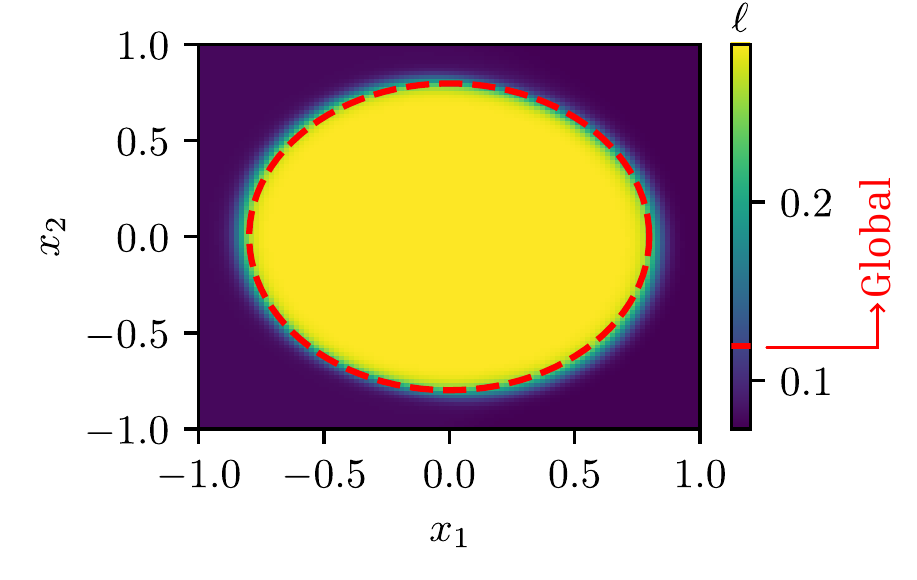
\includegraphics[width=1.0\textwidth]{figures/clustering/length_scale_2_500_0.png}
    \caption{Lengthscale hyperparameter in 2D. The colorplot indicates the smooth reconstruction while the red line in the colorbar the hyperparameter of a single global \gls{gp}.}
  \end{subfigure}
  \caption{Smooth reconstruction of the hyperparameters of the local \glspl{gp} using Eq.~\eqref{eq:clustering:smooth_hyper} for the non-stationary function defined in Eq.~\eqref{eq:clustering:function_nonstationary} in 1D (left) and 2D (right).}
  \label{fig:clustering:hyper_1d}
\end{figure}

In Fig.~\ref{fig:clustering:hyper_1d}, we show the smooth reconstruction of the hyperparameters of the local \glspl{gp} using Eq.~\eqref{eq:clustering:smooth_hyper} for the non-stationary function defined in Eq.~\eqref{eq:clustering:function_nonstationary} in 1D and 2D. In 1D, we show the kernel strength hyperparameter, while in 2D we show the length-scale hyperparameter. As we can see, in both cases the smooth reconstruction of the hyperparameters captures well the spatial variation of the function $f$. The kernel strength is high in the inner region where the amplitude of the cosine function is high, while it is low in the outer region where the amplitude is low. Similarly, the length-scale is high in the inner region where the frequency of the cosine function is low, while it is low in the outer region where the frequency is high. The hyperparameters of a single global \gls{gp} model are also shown for comparison. As we can see, they fail to capture any spatial variation and are an average over the entire input space.


{
\captionsetup[figure]{skip=4ex} % <--- <---
\captionsetup[subfigure]{skip=0ex} % <--- <---
\begin{figure}[htbp]
\begin{subfigure}{0.5\linewidth}
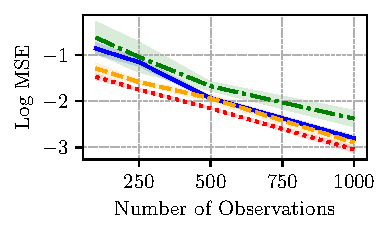
\includegraphics[width=\linewidth]{figures/clustering/error_comparison_dim_2.pdf}  % <---
  \caption{Average log-\gls{mse} in dimension 2.}
  \label{subfig:clustering:a_1}
\end{subfigure}
  \hfil
\begin{subfigure}{0.5\linewidth}
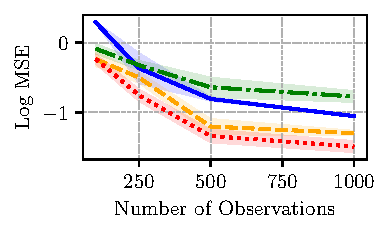
\includegraphics[width=\linewidth]{figures/clustering/error_comparison_dim_4.pdf} % <---
  \caption{Average log-\gls{mse} in dimension 4.}
  \label{subfig:clustering:b_1}
\end{subfigure}
\begin{subfigure}{0.5\linewidth}
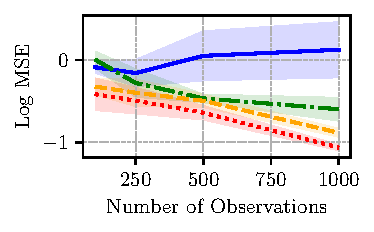
\includegraphics[width=\linewidth]{figures/clustering/error_comparison_dim_6.pdf}  % <---
  \caption{Average log-\gls{mse} in dimension 6.}
  \tikzmarknode{A}{}
  \label{subfig:clustering:a_2}
\end{subfigure}
  \hfil
\begin{subfigure}{0.5\linewidth}
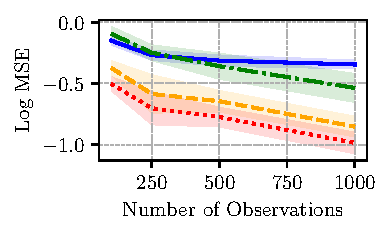
\includegraphics[width=\linewidth]{figures/clustering/error_comparison_dim_8.pdf} % <---
  \caption{Average log-\gls{mse} in dimension 8.}
  \tikzmarknode{B}{}
  \label{subfig:clustering:b_2}
\end{subfigure}
\begin{tikzpicture}[overlay, remember picture,
                  node distance=0ex and 0ex]
  \node (n1) [below  left=of $(A.south)!0.7!(B.south)$] {\scriptsize Global \gls{gp}};
  \draw[blue, very thick] (n1.west) -- ++ (-0.5,0) coordinate (aux1);
  \draw[orange,  very thick, dashed] (n1.east) -- ++ (+0.5,0) node (n2) [right] {\scriptsize \textcolor{black}{Clustered \gls{gp}}};
  \draw[green!50!black,  very thick, dashed] (n2.east) -- ++ (+0.5,0) node (n3) [right] {\scriptsize \textcolor{black}{\gls{dp}-\gls{gmm} Clustering}};
  \draw[red,  very thick, dashed] (n3.east) -- ++ (+0.5,0) node (n4) [right] {\scriptsize \textcolor{black}{Oracle.}};
  \node[draw, inner ysep=1pt, fit = (aux1) (n4)] {};
\end{tikzpicture}
\caption{Comparison of the average \gls{mse} for the global \gls{gp} model, the model-cluster \gls{gp}, a \gls{dp}-\gls{gmm} \gls{gp} and an oracle (which uses the exact clustering). Shaded regions indicate the $2\sigma$ confidence interval. }
\label{fig:clustering:tc3_post}
  \end{figure}
}

In Fig.~\ref{fig:clustering:tc3_post}, we compare the average \gls{mse} for the global \gls{gp} model on an independent test set between a single \gls{gp} model and a clustered \gls{gp} model (using the smooth reconstruction) for different number of observations and different dimensionalities of the input space. As we can see, the clustered \gls{gp} model consistently outperforms the single global \gls{gp} model, and its predictive capabilities are very close to the ones of oracle. In low dimensions, the global \gls{gp}'s performance is comparable (and sometimes even superior) to the one of the \gls{dp}-\gls{gmm} \gls{gp}. This is expected since the function is smooth and, although not ideal, a single \gls{gp} is still capable of interpolating the function. In higher dimensions, the performance of the global \gls{gp} becomes much worse.


\subsection{Results: Polynomial Expansion}
We now apply the clustering algorithm using polynomial expansions as local regressors, similarly to what we did in the previous example. Also in this case, the complex structure of the function $f$, defined in Eq.~\eqref{eq:clustering:function_nonstationary}, motivates the use of a clustering approach, as a single global polynomial would struggle to capture the behavior of $f$ across the entire domain. We use a polynomial expansion with Hermite polynomials of total degree $2$, selecting the coefficients by minimizing the \gls{mse} between the polynomial approximation and the observations. The clustering algorithm is run with $L^{(0)}=10$ initial clusters and an initial temperature of $T^{(0)}=1$.

\begin{figure}[htbp]
  \begin{subfigure}{0.49\linewidth}
    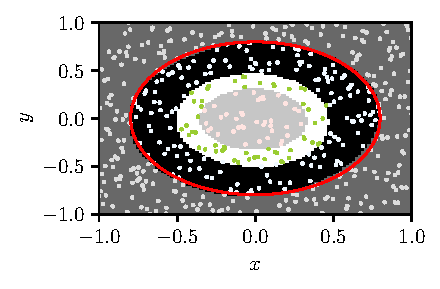
\includegraphics[width=1.0\textwidth]{figures/clustering/cluster_final_poly_tc2.pdf}
    \caption{Final clustering for the polynomial expansion.}
  \end{subfigure}
  \hfill
  \begin{subfigure}{0.49\linewidth}
    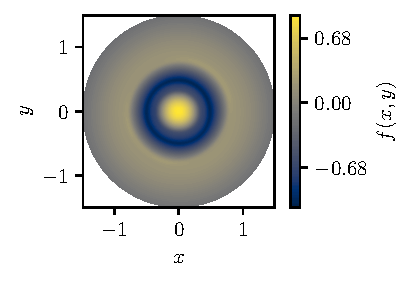
\includegraphics[width=1.0\textwidth]{figures/clustering/prediction_tc2_poly.pdf}
    \caption{Smooth reconstruction using the clustered polynomial expansion.}
  \end{subfigure}
  \caption{Final clustering and smooth reconstruction for the polynomial expansion applied to the non-stationary function.}
  \label{fig:clustering:poly_expansion_tc2}
\end{figure}

In Fig.~\ref{fig:clustering:poly_expansion_tc2}, we show the final clustering and the smooth reconstruction of the function $f$ using the clustered polynomial expansion. Also in this case the algorithm is able to identify the transition region of the function and to reconstruct the two regimes effectively. It is worth noting that the final number of clusters is higher than the actual number of regimes. In particular, the inner region has been split into 3 clusters arranged in a sort of concentric pattern. This split is necessary as we are using a polynomial expansion of degree $2$ as local regressor, which is not flexible enough to capture the behavior of the function in the entire inner region. The algorithm automatically detects this issue and splits the inner region into multiple clusters, allowing the local polynomial expansions to capture the behavior of the function more effectively. The same split is not observed in the outer region, due to the low number of observations and the difficulty of fitting a polynomial expansion in that region, which leads to the algorithm merging all the points in a single cluster.

\section{Example 3: Stick-Slip Oscillator}
\label{sc:tc3}

This last test case models a classic one-dimensional stick-slip oscillator: a mass, attached to a fixed support via a spring and a damper, and resting on a moving conveyor belt with a constant speed. The equation of motion is governed by the following ODE~\cite{stickslip},

\begin{equation}
    m \ddot{x} + c \dot{x} + k x = F_{\text{fric}}(v_{\text{rel}})\;.
\end{equation}

The quantity $x$ is the displacement of the mass relative to the fixed support, $\dot{x}$ is its absolute velocity, $m = 1.0$~kg is the mass, $c$ is the variable viscous damping coefficient, $k = 10.0$~N/m is the spring stiffness, and $v_{\text{rel}} = v - \dot{x}$ is the relative velocity between the constant belt speed $v$ and the mass velocity $\dot{x}$. The friction force $F_{\text{fric}}$ acting between the mass and the belt is modeled using the Stribeck law:

\begin{equation}
    F_{\text{fric}}(v_{\text{rel}}) = F_n \left[ \mu_k + (\mu_s - \mu_k) \exp\left(-\frac{|v_{\text{rel}}|}{v_s}\right) \right] \text{sgn}(v_{\text{rel}})
\end{equation}


where $F_n = 10.0$~N is the normal force, $\mu_s = 0.4$ is the static friction coefficient, $\mu_k = 0.2$ is the kinetic friction coefficient, and $v_s = 1.0$~m/s is the Stribeck characteristic velocity. 

\begin{figure}[htbp]
  \centering
  \begin{tikzpicture}[>=Stealth, thick]

% 1. Fixed Wall (Left)
\fill[pattern=north east lines] (-3, -0.5) rectangle (-2.5, 2.5);
\draw[thick] (-2.5, -0.5) -- (-2.5, 2.5);

% 2. Moving Conveyor Belt (Bottom)
\fill[gray!10] (-2.5, -1) rectangle (3.5, -0.5);
\draw[thick] (-2.5, -0.5) -- (3.5, -0.5); % Belt surface
\draw[thick] (-2.5, -1) -- (3.5, -1);     % Belt bottom
% Belt velocity vector
\draw[->, very thick, red!80!black] (1.5, -0.75) -- (2.5, -0.75) node[right] {$v$};

% 3. The Mass
\draw[thick, fill=blue!5] (0, -0.5) rectangle (2, 1.5);
\node at (1, 0.5) {\Large $m$};

% 4. Spring (Top parallel branch)
\draw[decoration={zigzag, pre length=0.6cm, post length=0.6cm, segment length=6pt, amplitude=5pt}, decorate] 
    (-2.5, 1) -- (0, 1);
\node[above] at (-1.25, 1.2) {$k$};

% 5. Damper (Bottom parallel branch)
% Cylinder attached to the wall
\draw (-2.5, 0) -- (-1.5, 0);       % Rod to wall
\draw (-1.5, 0.2) -- (-1.5, -0.2);  % Back of cylinder
\draw (-1.5, 0.2) -- (-0.7, 0.2);   % Top of cylinder
\draw (-1.5, -0.2) -- (-0.7, -0.2); % Bottom of cylinder
% Piston attached to the mass
\draw (0, 0) -- (-1.1, 0);          % Piston rod
\draw (-1.1, 0.15) -- (-1.1, -0.15);% Piston head
\node[below] at (-1.25, +0.8) {$c$};

% 6. Coordinates and Kinematics
% Zero-reference and displacement vector
\draw[dashed, thin] (1, 1.5) -- (1, 2);
\draw[->] (1, 1.8) -- (2, 1.8) node[right] {$x, \dot{x}$};

% 7. Friction Force
% Acting at the interface between the mass and the belt
\draw[->, very thick, orange!90!black] (1.0, -0.5) -- (-0.3, -0.5) node[above, yshift=-2pt] {$F_{\text{fric}}$};

\end{tikzpicture}
  \caption{Schematic of the stick-slip oscillator system.}
  \label{fig:clustering:stick_slip_oscillator}
\end{figure}

Fig.~\ref{fig:clustering:stick_slip_oscillator} illustrates the stick-slip oscillator system. The initial value problem is solved using a fourth-order Runge-Kutta (RK4) integration scheme with a fixed time step of $dt = 10^{-3}$~s. The initial conditions are set the equilibrium point of the system, i.e., $x(0) = F_{\text{fric}}(v_{\text{belt}})/k$ and $\dot{x}(0) = 0$. A small amount of noise is added to the initial conditions to trigger the oscillations. The system is simulated until a steady-state is reached, and the amplitude of the oscillations are computed as a QoI. The input parameters of interest are the belt velocity $v$ and the damping coefficient $c$. 


\begin{figure}[htbp]
\begin{subfigure}[t]{0.5\linewidth}
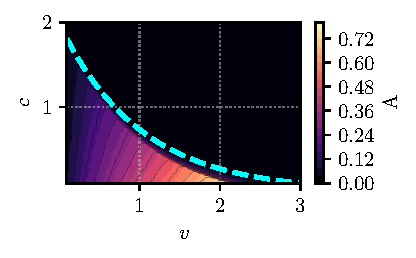
\includegraphics[width=\linewidth]{figures/clustering/stick_slip_contour.pdf}  % <---
  \caption{Oscillation amplitude at steady state. The dashed blue line indicates the critical transition from smooth sliding to stick-slip oscillations.}
  \tikzmarknode{A}{}
  \label{subfig:clustering:a_4}
\end{subfigure}
  \hfil
\begin{subfigure}[t]{0.5\linewidth}
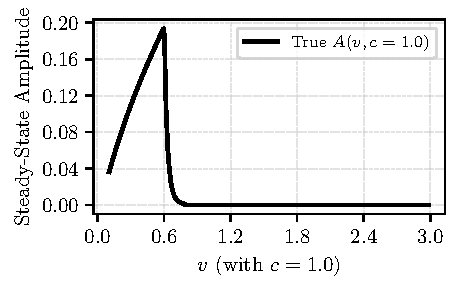
\includegraphics[width=\linewidth]{figures/clustering/function_profile_c_eq_v.pdf} % <---
  \caption{Oscillation amplitude profile along the line where $c = 1$. }
  \tikzmarknode{B}{}
  \label{subfig:clustering:b_4}
\end{subfigure}
\caption{Contour plot of the oscillation amplitude at steady state as a function of the belt velocity $v$ and the damping coefficient $c$ (left) and oscillation amplitude profile along the line where $c = 1$ (right). The dashed blue line in the left panel indicates the critical transition from smooth sliding to stick-slip oscillations.}
\label{fig:clustering:tc3_contour}
  \end{figure}


Fig.~\ref{fig:clustering:tc3_contour} shows the contour plot of the oscillation amplitude at steady state as a function of the belt velocity $v$ and the damping coefficient $c$ (left) and the oscillation amplitude profile along the line where $c = 1$ (right). Observing the two plots, increasing the belt velocity from zero leads to appearance of oscillations with increasing amplitude. At a critical belt velocity, the system becomes critically damped and the amplitude of the oscillations quickly drops to zero and the system enters the smooth sliding regime. The critical belt velocity at which this transition occurs is indicated by the dashed blue line in the left panel of Fig.~\ref{fig:clustering:tc3_contour}. The transition is abrupt but smooth.


\smallskip
The interest is to identify the different regimes of the system, i.e., the smooth sliding regime, the bifurcation transition, and the stick-slip oscillation regime, as a function of the input parameters $v$ and $c$. To this end we apply the clustering algorithm using \glspl{gp} with anisotropic elliptic Mat\'ern 5/2 kernel and constant mean function as local regressors. Furthermore, we use a \gls{dp}-\gls{gmm} to perform the initial clustering, as done by~\cite{Sudret2023}. After the initial clustering, we run just a few iterations of the clustering algorithm in the deterministic regime.

\begin{figure}[htbp]
\begin{subfigure}{0.5\linewidth}
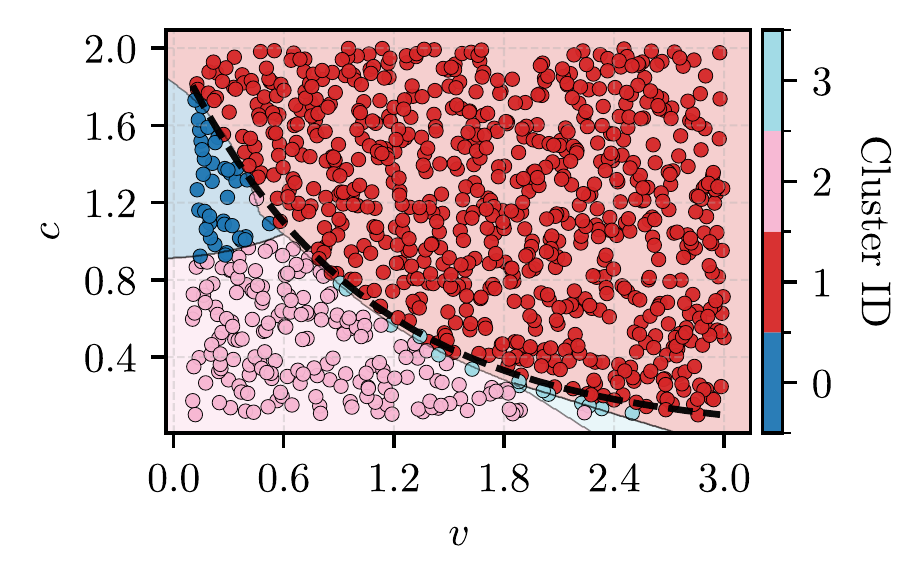
\includegraphics[width=\linewidth]{figures/clustering/cluster_plot_1000_0.png}  % <---
  \caption{Initial \gls{dp}-\gls{gmm} clustering.}
  \tikzmarknode{A}{}
  \label{subfig:clustering:a_5}
\end{subfigure}
  \hfil
\begin{subfigure}{0.5\linewidth}
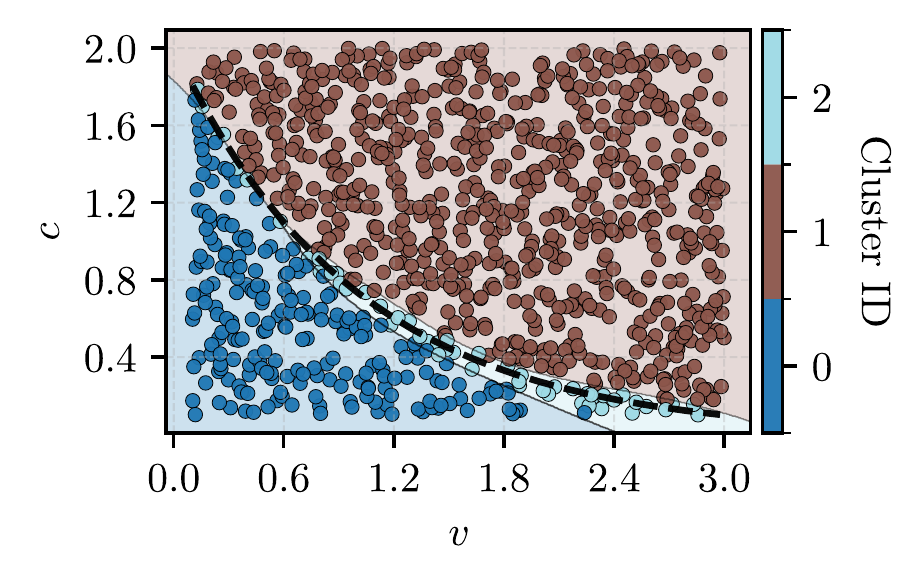
\includegraphics[width=\linewidth]{figures/clustering/cluster_plot_1000.png} % <---
  \caption{Final clustering after 75 iterations.}
  \tikzmarknode{B}{}
  \label{subfig:clustering:b_5}
\end{subfigure}
\caption{Clustering results at different iterations (1000 observations). (a) Initial \gls{dp}-\gls{gmm} clustering. (b) Final clustering after 75 iterations. Shaded regions correspond to the reconstructed subdomains $\hat{\Omega}_k$. The dashed line indicates the critical belt velocity.}
\label{fig:clustering:tc3_clusters_1}
\end{figure}

In Fig.~\ref{fig:clustering:tc3_clusters_1}, we show the clustering results at different iterations for $1000$ observations. The initial \gls{dp}-\gls{gmm} clustering (left) identified 4 clusters and correctly separated the smooth sliding regime from the stick-slip oscillation regime. However, our clustering algorithm is able to eliminate a redundant cluster in the stick-slip oscillation regime and expand the cluster in the bifurcating regime, leading to an improved clustering (right). 

\begin{figure}[htbp]
\begin{subfigure}{0.5\linewidth}
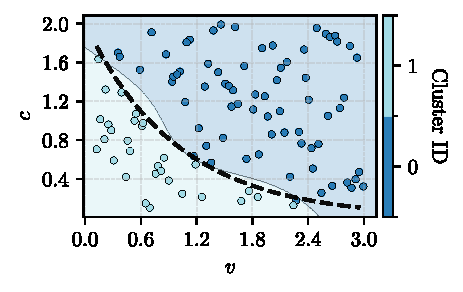
\includegraphics[width=\linewidth]{figures/clustering/cluster_plot_100.pdf}  % <---
  \caption{Final clustering with 100 observations.}
  \tikzmarknode{A}{}
  \label{subfig:clustering:a_6}
\end{subfigure}
  \hfil
\begin{subfigure}{0.5\linewidth}
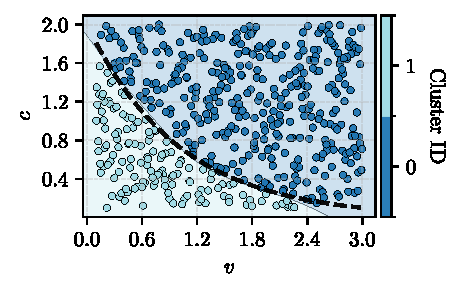
\includegraphics[width=\linewidth]{figures/clustering/cluster_plot_500.pdf} % <---
  \caption{Final clustering with 500 observations.}
  \tikzmarknode{B}{}
  \label{subfig:clustering:b_6}
\end{subfigure}
\caption{Final clustering for different number of observations. (a) Final clustering with 100 observations. (b) Final clustering with 500 observations. Shaded regions correspond to the reconstructed subdomains $\hat{\Omega}_k$. The dashed line indicates the critical belt velocity.}
\label{fig:clustering:tc3_clusters_2}
\end{figure}

If we reduce the number of observations to $100$ (left panel of Fig.~\ref{fig:clustering:tc3_clusters_2}) or $500$ (right panel of Fig.~\ref{fig:clustering:tc3_clusters_2}), the clustering algorithm is not able to identify the transition region and splits it into the two neighboring regimes. This is expected as the transition region is very narrow and a low number of observations may not be sufficient to capture it. However, even in these cases, the clustering algorithm is able to identify the two main regimes of the system, i.e., the smooth sliding regime and the stick-slip oscillation regime.


\subsection{Uncertainty Quantification}

To demonstrate the practical utility of the clustering framework for \gls{uq} studies, we assume that the input parameters follow distributions concentrated near the bifurcation regime and forward-propagate the uncertainty using the clustered \gls{gp} surrogate.

\begin{table}[htbp]
  \centering
  \begin{tabular}{lc}
    \toprule
    Parameter & Distribution  \\
    \midrule
    Belt velocity $v$ & $\mathcal{N}(1.2, 0.1^2)$  \\
    Damping coefficient $c$ & $\mathcal{N}(0.5, 0.1^2)$  \\
    \bottomrule
  \end{tabular}
  \caption{Parameter distributions for \gls{uq} analysis. Mean values situate the system near the critical bifurcation; standard deviations introduce variability across regimes.}
  \label{tab:uq_params}
\end{table}

We generate $10^4$ samples from the distributions specified in Table~\ref{tab:uq_params} and evaluate the oscillation amplitude QoI using the clustered and global \gls{gp} surrogates. 

\begin{figure}[htbp]
\centering
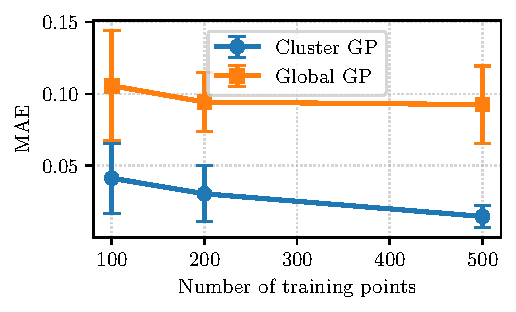
\includegraphics[width=0.6\textwidth]{figures/clustering/mae_vs_npoints_b.pdf}  % <---
\caption{\gls{mae} of the global \gls{gp} surrogate and the clustered \gls{gp} surrogate (using the smooth reconstruction) on the test set as a function of the number of training points.}
\label{fig:clustering:tc3_uq_1}
\end{figure}

In Fig.~\ref{fig:clustering:tc3_uq_1}, we show the \gls{mae} of the global \gls{gp} surrogate and the clustered \gls{gp} surrogate (using the smooth reconstruction) on the test set as a function of the number of training points. The clustered \gls{gp} surrogate consistently outperforms the global \gls{gp} surrogate, especially for low number of training points.

\smallskip
For a more practical demonstration, we now use the surrogate models to estimate the \gls{cdf} of the oscillation amplitude under the input uncertainty specified in Table~\ref{tab:uq_params}. The \gls{cdf} provides a complete estimate of the distribution of the QoI and is particularly informative for risk assessment and decision-making. To this end, we also estimate the probability $\mathbb{P}(A > 0.5)$, which quantifies the likelihood of observing oscillation amplitudes exceeding a critical threshold, a key metric for assessing the risk of severe stick-slip oscillations.

\smallskip
To be conservative, we do not use the mean prediction of the surrogate models to estimate the \gls{cdf} and the probability $\mathbb{P}(A > 0.5)$, but we use the 95\% \gls{ucb} of the surrogate models. First, for the global \gls{gp} surrogate, we can directly estimate the \gls{ucb} using the predictive mean and variable of the predictive distribution. For the clustered \gls{gp} surrogate, we estimate the \gls{ucb} using the \gls{gmm} reconstruction of the function. Indeed, the \gls{gmm} reconstruction preserves the, potentially discontinuous, transitions between the different regimes, while the smooth reconstruction (and similarly a single global \gls{gp}) will smooth out such transitions.


{
\captionsetup[figure]{skip=4ex} % <--- <---
\captionsetup[subfigure]{skip=0ex} % <--- <---
\begin{figure}[htbp]
\begin{subfigure}[t]{0.5\linewidth}
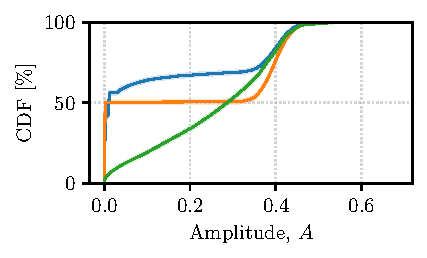
\includegraphics[width=\linewidth]{figures/clustering/amplitude_three_cdfs_with_ci.pdf}  % <---
  \caption{Estimated \gls{cdf} of the oscillation amplitude. Shaded regions correspond to the 95\% confidence interval of the \gls{cdf} estimates using a bootstrap procedure.}
  \tikzmarknode{A}{}
  \label{subfig:clustering:a_7}
\end{subfigure}
  \hfil
\begin{subfigure}[t]{0.5\linewidth}
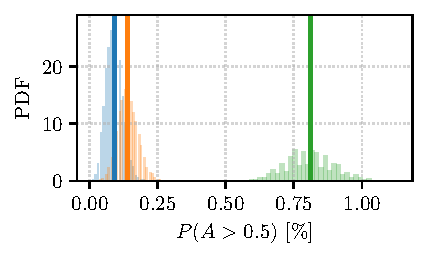
\includegraphics[width=\linewidth]{figures/clustering/probability_A_gt_0p5_three_distributions.pdf} % <---
  \caption{Estimated probability $\mathbb{P}(A > 0.5)$. The solid lines correspond to the point estimates while the histogram corresponds to the distribution of the estimates obtained using a bootstrap procedure.}
  \tikzmarknode{B}{}
  \label{subfig:clustering:b_7}
\end{subfigure}
\begin{tikzpicture}[overlay, remember picture,
                  node distance=0ex and 0ex]
  \node (n1) [below  left=of $(A.south)!0.8!(B.south)$] {\scriptsize True};
  \draw[blue, very thick] (n1.west) -- ++ (-0.5,0) coordinate (aux1);
  \draw[green!60!black,  very thick] (n1.east) -- ++ (+0.5,0) node (n2) [right] {\scriptsize \textcolor{black}{Global \gls{gp}}};
  \draw[orange,  very thick] (n2.east) -- ++ (+0.5,0) node (n3) [right] {\scriptsize \textcolor{black}{Clustered \gls{gp}}};
  \node[draw, inner ysep=1pt, fit = (aux1) (n3)] {};
\end{tikzpicture}
\caption{Estimated \gls{cdf} of the oscillation amplitude (left) and estimated probability $\mathbb{P}(A > 0.5)$ (right) using the global \gls{gp} surrogate and the clustered \gls{gp} surrogate. The true \gls{cdf} and probability are also shown for comparison. The number of training points used to train the surrogate models is $200$.}
\label{fig:clustering:tc3_uq_2}
  \end{figure}
}

In Fig.~\ref{fig:clustering:tc3_uq_2}, we show the estimated \gls{cdf} of the oscillation amplitude (left) and the estimated probability $\mathbb{P}(A > 0.5)$ (right) using the global \gls{gp} surrogate and the clustered \gls{gp} surrogate. It is clear that the clustered \gls{gp}, apart from being more accurate, provides an estimate of the \gls{cdf} that mimics well the true \gls{cdf}. It indeed captures the abrupt transition from sliding to stick-slip oscillations. On the other hand, the global \gls{gp} surrogate fails to capture such transition and smooths it out. While adding more points to train the global \gls{gp} surrogate can improve the accuracy, it will never be able to capture the abrupt transition and will always smooth it out. This is a clear demonstration of the practical utility of the clustering framework for \gls{uq} studies and highlights the different predictive methods (smooth vs \gls{gmm} reconstruction) that can be used to reconstruct the global function from the local models. Finally, the estimated probability $\mathbb{P}(A > 0.5)$ using the clustered \gls{gp} surrogate is much closer to the true probability than the estimate obtained using the global \gls{gp} surrogate. Both estimates correctly overestimate the true probability, which is expected as we are using the \gls{ucb} of the surrogate models to make the estimates.




\section{Conclusions and Future Perspectives}
\label{sc:conclusions}

In this chapter we have presented a novel domain decomposition approach for surrogate modeling of complex functions. The framework is based on a model-based clustering algorithm that using information from local surrogate models and a classifier, is able to cluster the input space into subdomains where the function is smooth and can be effectively approximated by a local surrogate model. We have developed an iterative algorithm that improves an initial clustering of the training data. The algorithm is based on a stochastic update rule that iteratively updates the membership assignments of the training data to maximize an appropriate score function. We then show that, under additional assumptions, the deterministic version of the algorithm terminates after a finite number of steps. For improved computational efficiency, we propose relaxing these assumptions; this may allow contained limit-cycle oscillations, a behavior that can be detected using a robust stopping criterion.

\smallskip
We leverage the information coming from the local regressors to reconstruct the global function using three different methods: a piecewise reconstruction that uses a hard partitioning of the input space, a smooth reconstruction that uses the probabilities of the classifier to weight the contribution of the local regressors, and a \gls{gmm} reconstruction that uses the same probabilities to build a mixture distribution from the local regressors' outputs. Each method has its own advantages and disadvantages, and the choice of the method to use depends on the specific problem at hand and on the desired properties of the global surrogate model. The piecewise reconstruction is simple and computationally efficient, but it can lead to discontinuities at the boundaries between the clusters. The smooth reconstruction can capture smooth transitions between the clusters, but it can also smooth out abrupt transitions. The \gls{gmm} reconstruction can capture both smooth and abrupt transitions.

\smallskip
The algorithm is model-agnostic and can be used with any regression model and any classification algorithm. We provided a complete guide on how to express the clustering objective function for \glspl{gp} and polynomial expansions as local regressors and \glspl{svm} as classifiers. In the test cases, for simplicity, we emphasized the use of \glspl{gp} as local regressors, with preliminary results also for polynomial expansions. The flexibility of the proposed approach makes it applicable to a wide range of problems in \gls{uq} and surrogate modeling.

\smallskip
We have demonstrated the effectiveness of the proposed approach on several comprehensive test cases. First, we dealt with a function with a mix of first and zeroth order discontinuities. We investigated how well the clustering algorithm is able to identify the different discontinuities across different dimensionalities of the input space and different number of observations. We also investigate how and why the algorithm can fail to identify the discontinuities and showed that, even in these cases, the resulting clustering still yields a lower \gls{mse} than a single global surrogate model. To this end, we also compared the behavior and the distribution of the \gls{mse} across multiple dimensionalities and different number of observations. The second test case dealt with a smooth function with an abrupt transition between two regimes. We showed that the clustering algorithm is able to identify the transition region and to reconstruct the two regimes effectively. Finally, we applied the proposed approach to a stick-slip oscillator, a classic problem in nonlinear dynamics. We showed that the clustering algorithm is able to identify the different regimes of the system, i.e., the smooth sliding regime, the bifurcation transition, and the stick-slip oscillation regime, as a function of the input parameters. We also demonstrated the practical utility of our clustering framework by using the \gls{gmm} distribution to estimate the \gls{cdf} of the oscillation amplitude under input uncertainty and to estimate the probability of observing oscillation amplitudes exceeding a critical threshold. As expected, the clustered \gls{gp} surrogate provided much more accurate estimates than the global \gls{gp} surrogate. Most importantly, the \gls{gmm} reconstruction was able to capture the abrupt transition from sliding to stick-slip oscillations, providing an estimate of the \gls{cdf} that mimics well the true \gls{cdf}, while the global \gls{gp} surrogate failed to capture such transition and smoothed it out.

\smallskip
\blue{The main limitation of the proposed approach is that it requires a sufficient number of observations to effectively identify the different regimes of the function. In cases where the number of observations is low, the clustering algorithm may fail to identify the transition regions and may merge different regimes into a single cluster. This can lead to a loss of accuracy in the global surrogate model. We firmly believe that this limitation can be tamed by combining our model-based clustering algorithm with an active learning strategy to enrich the training set. Such a strategy could potentially infill the input space with points that help improve the knowledge of boundaries and improve the local surrogate models.}

\smallskip
\blue{Furthermore, while capable of identifying the presence of a discontinuity, our clustering algorithm is not guaranteed to converge to the solution that has the lowest possible number of clusters. A simple merging strategy was proposed to merge clusters whose spatial regions are overlapping. This strategy is not robust as it may mistakenly merge clusters that are separated by a discontinuity (provided that the temperature is sufficiently high) or not merge clusters at all (if the temperature is too low). A possible research direction consists in investigating more robust merging strategies that can work also at low temperatures.}
